\documentclass[a4paper,fleqn]{__CAS_CLASS__}
\usepackage[authoryear,longnamesfirst]{natbib}
\usepackage{longtable,booktabs,array,calc}
\makeatletter
\providecommand\insert@pcolumn{\insert@column}
\makeatother
\providecommand{\tightlist}{%
  \setlength{\itemsep}{0pt}\setlength{\parskip}{0pt}}
\begin{document}
\shorttitle{Benchmarking of Embedding Models}
\shortauthors{Murat Karakaya}
\title[mode=title]{Benchmarking of Embedding Models}
\author[1]{Murat Karakaya}[orcid=TODO: 0000-0000-0000-0000]
\cormark[1]
\ead{murat.karakaya@tedu.edu.tr}
\affiliation[1]{organization={Department of Software Engineering, TED University},city={Ankara},country={T\"urkiye}}
\cortext[1]{Corresponding author}
\begin{abstract}
This study presents an end-to-end embedding benchmarking pipeline for evaluating embedding models on local datasets and selecting the best suitable model for specific application requirements in Retrieval-Augmented Generation workflows \citep{Lewis_RAG_2021}. The pipeline performs controlled multi-model evaluation, computes standard retrieval metrics (\texttt{MAP@10}, \texttt{Recall@10}, \texttt{Precision@10}, \texttt{NDCG@10}, \texttt{MRR@10}, \texttt{Success@10}), and generates well-structured dynamic report outputs (timestamped markdown/pdf plus visualizations) for practical decision support \citep{Aggregate_Report_2026_03_05}.

We demonstrate the pipeline with three datasets (\texttt{education\_eng}, \texttt{education\_tr}, \texttt{law\_tr}) curated from TED University regulations and BDDK legislation sources, and five sentence-transformer embedding models under a frozen configuration \citep{TED_Regulations, BDDK_Mevzuat, Raw_Education_Eng_2026_03_05, Raw_Education_Tr_2026_03_05, Raw_Law_Tr_2026_03_05}. Results show that embedding performance is language- and domain-dependent, and that quality-speed tradeoffs vary materially across models, so model choice should be fit-for-purpose rather than based on universal superiority claims \citep{Aggregate_Report_2026_03_05}. The pipeline and artifacts are released publicly to support reuse by developers \citep{GitHub_RagRetrievalBench}.

\end{abstract}
\begin{highlights}
\item A reusable local pipeline benchmarks embedding models for fit-for-purpose selection.
\item The pipeline generates automatic, structured reports with quality and operational metrics.
\item Validation on three datasets and five models shows dataset-dependent ranking differences.
\end{highlights}
\begin{keywords}
Embedding Benchmarking \sep Retrieval \sep Model Selection \sep Local Dataset \sep RAG
\end{keywords}
\maketitle
\section{Introduction}\label{introduction}

Retrieval-augmented generation (RAG) systems depend on retrieval quality to ground generated answers, so embedding-model choice directly affects downstream reliability. In operational settings, this choice is rarely made on generic benchmark corpora alone; it is made for local document collections whose language, domain vocabulary, document structure, and latency constraints may differ from public evaluation settings. A model that performs strongly in one context may therefore be less suitable when the deployment corpus changes. \citep{Lewis_RAG_2021}

Public leaderboards and informal local trials remain useful starting points, but they are insufficient as a complete basis for deployment decisions. Generic rankings do not reveal whether a model remains effective on a practitioner's own corpus, while ad hoc testing can confound model behavior with changes in preprocessing, query construction, relevance judgments, retrieval depth, or reporting criteria. Existing local evaluations also tend to treat key concerns separately: they may compare retrieval quality, report operational cost, or preserve reproducible artifacts, but they do not always combine shared-protocol model comparison, reusable benchmark evidence, language and domain comparability, quality--speed reporting, consistency diagnostics, and statistical decision support in one workflow. This gap motivates a controlled local benchmarking process that produces corpus-specific evidence for fit-for-purpose embedding selection rather than a universal model ranking.

This paper addresses that practical model-selection problem by presenting a reusable local benchmarking pipeline for embedding-model evaluation under corpus-specific RAG requirements. The pipeline transforms local document collections into controlled benchmark artifacts, evaluates candidate embedding models under one fixed protocol, and generates structured reports for retrieval effectiveness, operational behavior, cross-dataset consistency, and statistical decision support. Its intended output is decision support for practitioners: a way to compare candidate models transparently, preserve the underlying raw evidence, and regenerate dataset-level or aggregate reports when the evaluation context changes. \citep{GitHub_RagRetrievalBench}

The pipeline is demonstrated through a fixed experimental snapshot covering three document collections and five embedding models. The snapshot contains 60 source documents, 1{,}914 chunks, 150 synthetic queries, and 952 positive query--chunk relevance judgments (qrels, the ground-truth labels that mark which chunks are relevant to each query), providing a compact but heterogeneous test bed for examining language sensitivity, domain sensitivity, and operational tradeoffs. The broader questions of language and domain sensitivity are instantiated through English and Turkish education corpora and through Turkish education and law/regulation corpora, while operational decision support is instantiated through shared retrieval-quality, timing, consistency, and statistical outputs. Setup details, including provenance and controlled parameters, are provided in Section~\ref{experiments}; quantitative comparative evidence is reported in Section~\ref{results}.

\paragraph{Contributions and Research Questions}\label{contributions}
The paper makes four contributions to local RAG benchmarking practice. First, it defines a reusable pipeline for corpus-specific embedding-model selection under a controlled evaluation frame. Second, it integrates automatic report generation that consolidates retrieval quality, operational measurements, consistency diagnostics, and statistical outputs into decision-support artifacts. Third, it supports cross-dataset comparability through shared protocol execution and aggregate reporting. Fourth, it provides a publicly accessible implementation and benchmark artifacts to improve reuse and reproducibility in practitioner workflows. \citep{GitHub_RagRetrievalBench}

\paragraph{Research Questions}\label{research-questions}
Guided by these contributions, the empirical analysis addresses four broad research questions:

\begin{itemize}
\tightlist
\item
  RQ1 (Pipeline utility): Can the pipeline produce decision-support evidence---a ranked model shortlist with retrieval-quality metrics, operational-cost measurements, and query-level uncertainty estimates---for embedding-model selection on a local document collection?
\item
  RQ2 (Language sensitivity): Under one fixed benchmark protocol, can the pipeline expose language-conditioned ranking changes within this bounded snapshot?
\item
  RQ3 (Domain sensitivity): Under one fixed benchmark protocol, can the pipeline expose domain-conditioned ranking changes within this bounded snapshot?
\item
  RQ4 (Operational decision support): How does the pipeline combine retrieval effectiveness, operational cost, and query-level uncertainty into fit-for-purpose deployment guidance?
\end{itemize}

To make these questions answerable rather than rhetorical, we fix the operational meaning of the terms used throughout the paper. \emph{Decision-support evidence} (used interchangeably with \emph{actionable evidence}) is a per-model summary---retrieval-quality metrics, query latency and indexing throughput, and query-level uncertainty intervals---that is sufficient to choose a model under a stated deployment priority such as quality-first or latency-first. \emph{Pipeline utility} (RQ1) is the pipeline's ability to produce such a summary reproducibly from a local corpus while preserving the underlying raw artifacts. \emph{Consistency diagnostics} are the cross-condition stability summaries defined in Section~\ref{results} (all-metric coefficient of variation, worst-case metric drop, and score range). \emph{Statistical decision support} is the query-level bootstrap confidence-interval layer that indicates whether an observed difference is distinguishable from sampling noise, and it replaces inferential tests computed over only three dataset-level means.

These research questions are intentionally framed at the level of local benchmarking practice, but the empirical claims in this paper are bounded to the fixed experimental snapshot reported here. The evaluated evidence comes from three curated document collections, two languages, two domain settings, five embedding models, and one controlled retrieval configuration. Therefore, the paper does not claim universal model superiority. Instead, it evaluates whether the proposed workflow can produce reliable, reusable, and decision-relevant evidence for fit-for-purpose embedding-model selection under controlled local conditions.

Section~\ref{related-work} positions the paper against prior work, Section~\ref{method} describes the proposed workflow, Section~\ref{experiments} documents the experimental setup, Section~\ref{results} reports comparative evidence, and Section~\ref{conclusion} concludes with implications and future directions.

\section{Related Work}\label{related-work}

\subsection{RAG Retrieval Evaluation and Embedding Benchmarking}\label{rag-retrieval-evaluation-and-embedding-benchmarking}

RAG systems depend on retrieval quality to maintain answer grounding and downstream reliability, so retrieval design remains a central determinant of end-task behavior. Foundational work establishes this dependency, and later survey evidence frames retrieval as a multi-component design space spanning query processing, retrieval, reranking, and generation-time integration. \citep{Lewis_RAG_2021, Zhu_LLMIR_Survey_2025}

Recent applied studies reinforce this point in domain-specific settings. Knowledge-graph-augmented RAG pipelines for cybersecurity and customs support report that retrieval-side design choices materially affect answer quality and contextual relevance. \citep{Gao_KG_RAG_Power_2025, Hu_ICCARAG_2025} QuIM-RAG further demonstrates that retrieval-oriented query matching strategies can improve question-answering effectiveness relative to simpler baseline retrieval flows. \citep{Saha_QuIMRAG_2024}

Related evidence from question-retrieval research also indicates that metadata-aware retrieval strategies can improve ranking quality in practical question-answering environments, which is consistent with the broader claim that retrieval quality is highly configuration-sensitive. \citep{Ghasemi_Metadata_QR_2024}

Taken together, these studies motivate retrieval-aware system design, but they are typically optimized for one task setting or one domain-specific application pipeline. In contrast, this paper focuses on controlled cross-dataset embedding-model selection under a fixed evaluation protocol, with reusable benchmark artifacts and reporting outputs intended for practitioner-facing local deployment decisions.

\subsection{Preliminary Conference Study (Short Context)}\label{preliminary-conference-study-short-context}

Our earlier conference paper (\texttt{publishedConferencePaper.pdf}) introduced a local automated benchmark pipeline and demonstrated it on a single technical English corpus. That preliminary work established feasibility for end-to-end automated evaluation with synthetic queries, LLM-based qrels, and multi-model retrieval metrics. \citep{Karakaya_Conference_2025}

\subsection{Extension in the Current Journal Work}\label{extension-in-the-current-journal-work}

This journal paper extends the preliminary work in scope and practical selection value: it uses a frozen cross-dataset setup with \texttt{education\_eng}, \texttt{education\_tr}, and \texttt{law\_tr}, and evaluates 5 embedding models under one consistent pipeline configuration. The dataset sources are explicitly documented (TED regulations/guidelines for education datasets and BDDK regulations for law dataset, retrieved on 01/01/2026). The extension adds aggregate cross-dataset ranking, consistency analysis, and quality-speed analysis, plus automatic benchmarking reports across various metrics, to support cross-dataset comparison for dataset-specific model selection. \citep{Aggregate_Report_2026_03_05, Raw_Education_Eng_2026_03_05, Raw_Education_Tr_2026_03_05, Raw_Law_Tr_2026_03_05, TED_Regulations, BDDK_Mevzuat}

In short, the conference paper is context only; the journal evidence is driven by the current multi-dataset artifacts and emphasizes that the pipeline is reusable by practitioners for choosing the most suitable embedding model for application requirements. \citep{Karakaya_Conference_2025, GitHub_RagRetrievalBench}

\section{Method}\label{method}

This study proposes a reusable local benchmarking pipeline for selecting embedding models under corpus-specific Retrieval-Augmented Generation (RAG) requirements. The method is organized as a staged workflow that transforms local document collections into controlled benchmark artifacts, including chunked corpora, synthetic queries, relevance judgments, model-specific vector indexes, and structured reporting outputs. Each intermediate artifact serves as a controlled input to the next stage, which allows candidate embedding models to be evaluated under the same benchmark evidence rather than under model-specific or manually curated test sets. This design supports both single-dataset model selection and, when heterogeneous corpus subsets are benchmarked separately, aggregate comparison across topic- or language-specific dataset partitions.

\subsection{Pipeline Overview}\label{pipeline-overview}

The pipeline operates at the dataset level and begins with explicit dataset routing, as illustrated in Figure~\ref{fig:method_pipeline_workflow}. Each corpus is processed in isolation so that document inputs, chunked corpora, synthetic queries, qrels, vector collections, and reports remain separated across datasets. This design reduces cross-dataset contamination and allows the same methodological template to be applied repeatedly to document collections that differ in language, domain, and scale. After routing, the workflow advances through document ingestion, chunking, query generation, and relevance construction, thereby producing the benchmark artifacts required for comparative retrieval.

Once these shared artifacts have been created, the pipeline branches into model-specific indexing and evaluation. Separate vector collections are built for each candidate embedding model, and each model is evaluated against the same query and qrels resources rather than against model-specific or manually curated evidence. The final stage consolidates the resulting outputs into dataset-level reports and, when multiple corpora are available, into an aggregate comparison report. The sequence of stages and their intermediate products are summarized in Table~\ref{tbl:method_pipeline_stages} and illustrated conceptually in Figure~\ref{fig:method_pipeline_workflow}.

\begin{table}[t]
\caption{Stage sequence and intermediate artifacts of the proposed embedding benchmarking workflow.}\label{tbl:method_pipeline_stages}
\centering
\small
\begin{tabular}{@{}>{\raggedright\arraybackslash}p{0.14\linewidth}>{\raggedright\arraybackslash}p{0.16\linewidth}>{\raggedright\arraybackslash}p{0.38\linewidth}>{\raggedright\arraybackslash}p{0.22\linewidth}@{}}
\toprule
Stage & Input & Process & Output \\
\midrule
Dataset routing & Local dataset selection & Bind one dataset to isolated working paths so downstream artifacts remain separated across corpora & Dataset-specific run context \\
Document ingestion & Routed document collection & Parse source documents and normalize extracted text for downstream processing & Textual corpus \\
Chunking & Textual corpus & Segment documents into overlapping units suitable for embedding and retrieval & Chunked corpus \\
Query generation & Chunked corpus & Sample seed chunks and generate natural-language queries in the source language of the seed content & Synthetic query set \\
Relevance construction & Query set and chunked corpus & Retrieve a bounded candidate pool for each query and assign binary relevance labels through LLM-assisted judgment & Qrels resource \\
Multi-model indexing & Chunked corpus and selected embedding models & Build a separate vector collection for each embedding model so retrieval runs remain isolated and reproducible & Per-model vector collections \\
Retrieval evaluation & Query set, qrels, and per-model collections & Execute the same fixed-depth retrieval workflow for every model over the same benchmark artifacts & Ranking artifacts and timing traces \\
Reporting & Dataset-level evaluation artifacts & Produce dataset-level reports and aggregate comparison artifacts for downstream interpretation & Benchmark reports and visual summaries \\
\bottomrule
\end{tabular}
\end{table}

\begin{figure}
\centering
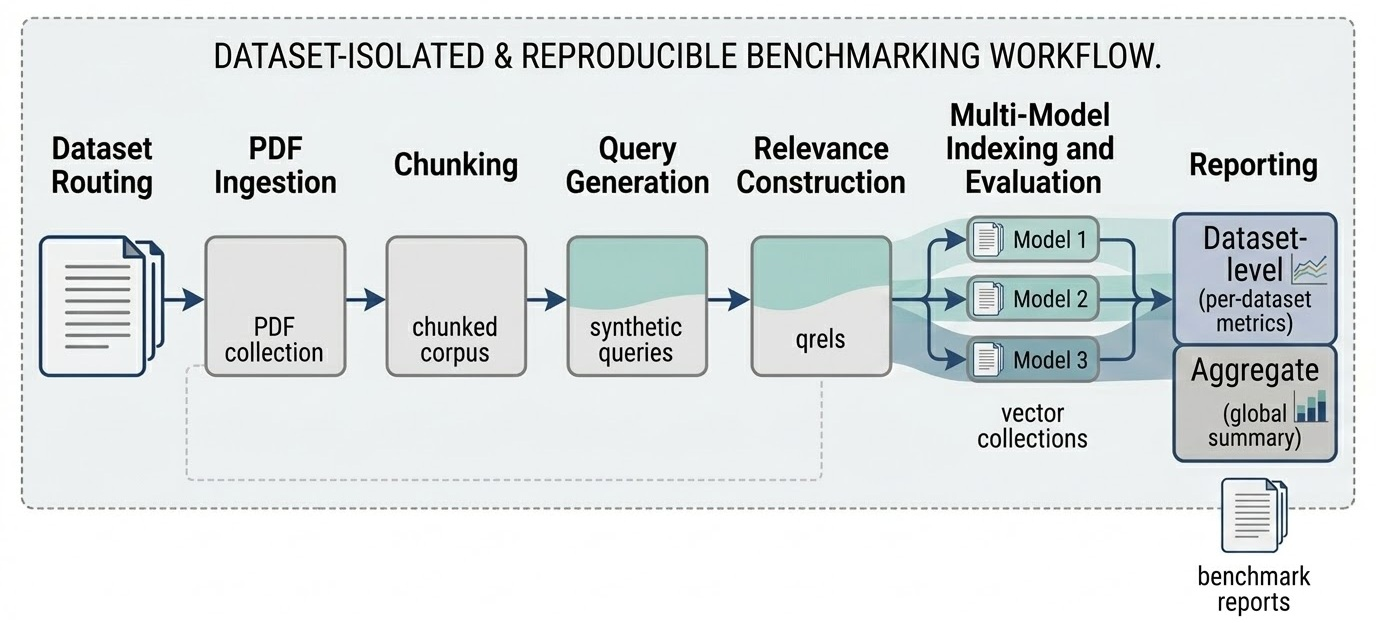
\includegraphics[width=0.95\linewidth]{conceptual_overview.jpg}
\caption{Conceptual overview of the proposed embedding benchmarking pipeline.}\label{fig:method_pipeline_workflow}
\end{figure}

\subsection{Corpus Preparation}\label{corpus-preparation}

The first stage converts each local document collection into a benchmarkable text corpus. Source documents are ingested from the local corpus and parsed into textual segments; in the present experimental snapshot, these source documents are provided as PDF files. To preserve local context while keeping units manageable for downstream embedding models, the extracted text is segmented by recursive character-based chunking with controlled overlap between adjacent segments. This strategy reduces the probability that semantically dependent passages are split into entirely disconnected units, while still producing retrieval items that can be embedded and indexed efficiently. The fixed parameterization used in the experimental instantiation of this workflow is summarized in Section~\ref{shared-evaluation-setup}.

Dataset-level isolation is maintained during corpus preparation. Each dataset yields its own chunked corpus and retains its own storage path for downstream artifacts. As a result, the same pipeline can be reused across multiple corpora without mixing documents, collections, or reports between experiments.

\subsection{Synthetic Query and Relevance Construction}\label{synthetic-query-and-relevance-construction}

After corpus construction, the pipeline constructs benchmark queries and relevance judgments through the sequence shown in Figure~\ref{fig:method_qrels_workflow}. Each instance begins with a seed chunk sampled from the corpus. Rather than relying on externally authored questions, the method prompts a large language model to generate a concise natural-language query in the same language as that sampled chunk. In this sense, the pipeline uses the language model as a query-construction judge that converts one corpus-grounded seed passage into one evaluation query while preserving the linguistic and topical characteristics of the underlying dataset. This design keeps query formulation anchored to the target corpus while avoiding the cost of manually preparing a query set for each new dataset.

Relevance construction then proceeds from the generated query. The system retrieves a bounded candidate pool of corpus chunks, with the candidate set size fixed by the shared experimental configuration summarized in Section~\ref{shared-evaluation-setup}, and presents these query--chunk pairs to the language model for binary relevance labeling. The same LLM-as-judge principle is therefore used a second time, now to decide whether each candidate chunk is relevant to the generated query and should be retained in the qrels resource for later retrieval evaluation. The output of this stage is not a free-form annotation record, but a qrels artifact in which candidate passages are marked as relevant or non-relevant under a consistent automated judgment procedure. Because the query set and qrels are created before comparative model assessment begins, all embedding models are evaluated against the same benchmark artifacts under a controlled protocol.

\begin{figure}
\centering
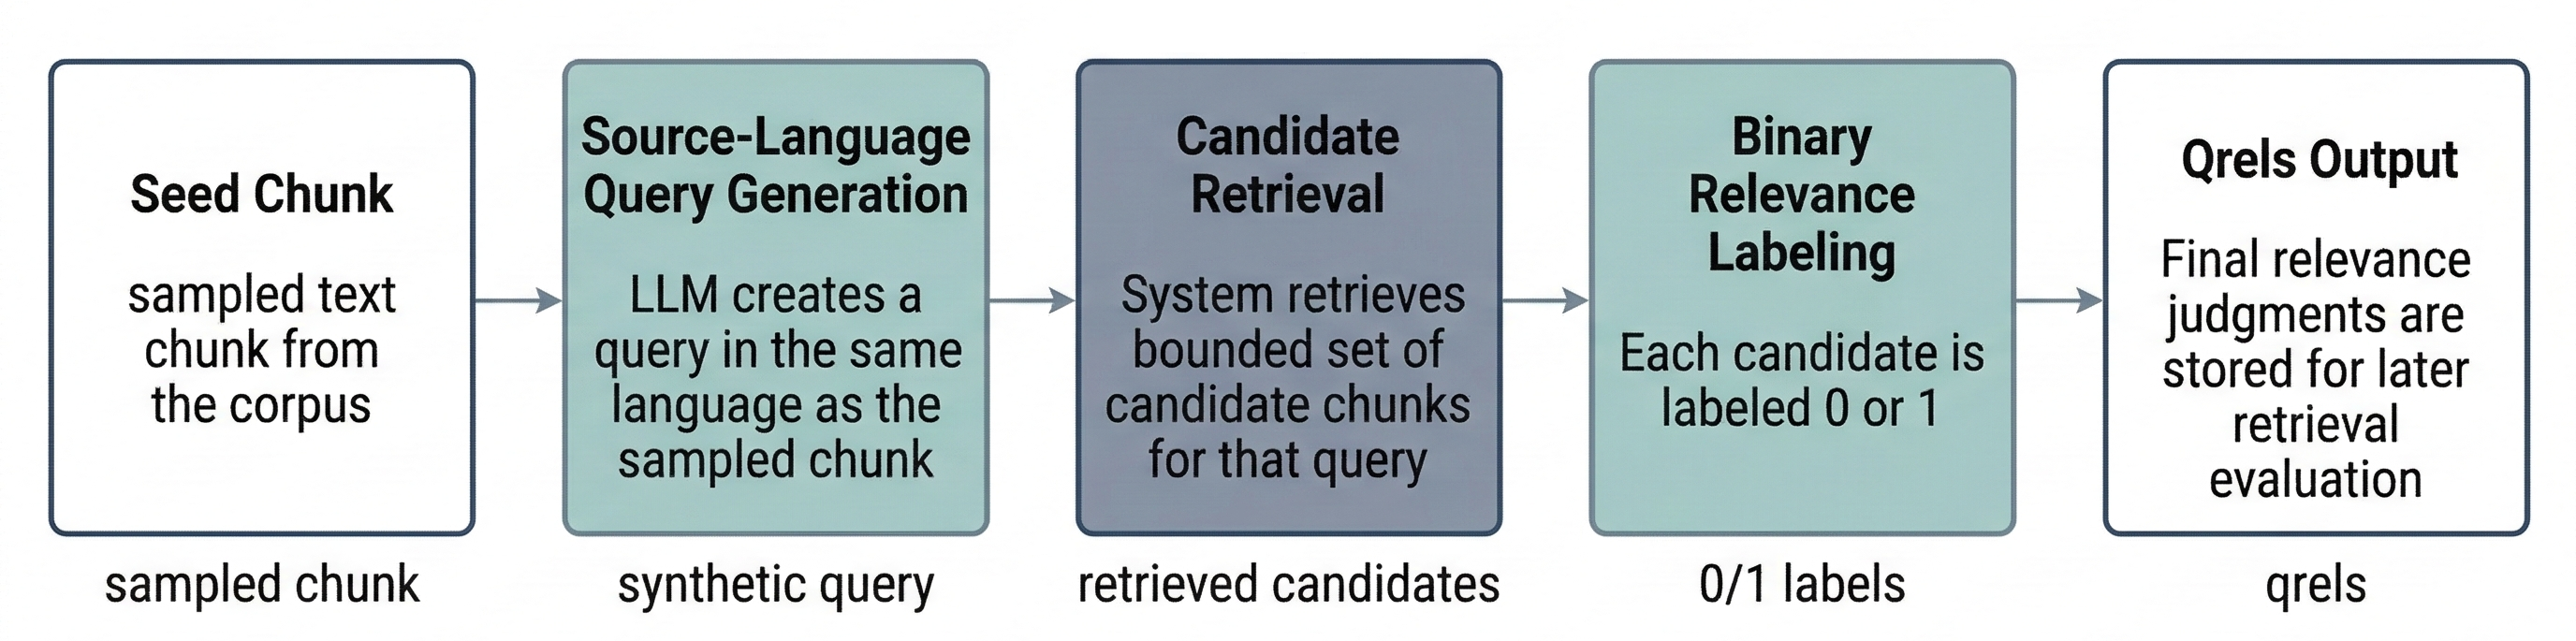
\includegraphics[width=0.95\linewidth]{query_qrels.png}
\caption{Workflow for synthetic query generation and binary relevance construction.}\label{fig:method_qrels_workflow}
\end{figure}

\subsection{Embedding Index Construction}\label{embedding-index-construction}

The comparative evaluation stage uses a fixed set of sentence-transformer models spanning lightweight, higher-capacity, and multilingual alternatives within a single benchmarking design. Each model is assigned its own vector collection so that embedding generation, storage, and retrieval remain isolated across models. This separation is methodologically important because it ensures that observed differences arise from the embedding models themselves rather than from shared or overwritten index state. The exact benchmarked model roster is specified in the experimental setup. \citep{SentenceTransformers_Pretrained}

Model-specific collections are built from the same chunked corpus. This means that corpus content, query set, and relevance judgments remain fixed while only the embedding function changes across runs. Such control is necessary if the benchmark is to support fit-for-purpose model selection rather than confound model comparison with changes in the evaluation dataset itself.

\subsection{Retrieval Evaluation Workflow}\label{retrieval-evaluation-workflow}

Once the vector collections are initialized, the pipeline executes the retrieval loop shown in Figure~\ref{fig:method_retrieval_workflow}. Each evaluation instance begins with a synthetic query drawn from the shared benchmark set. That query is submitted to a model-specific ChromaDB collection, where the embedding model under evaluation determines the vector representation used for search. The system then returns a ranked list of retrieved chunks under a fixed cutoff, ensuring that every model is tested at the same retrieval depth. The shared evaluation settings that constrain this loop are summarized in Section~\ref{shared-evaluation-setup}. \citep{ChromaDB_Docs}

The ranked results are subsequently aligned with the previously constructed qrels so that each query is interpreted against the same binary relevance resource, regardless of which embedding model produced the ranking. This ordering is methodologically important because corpus segmentation, query construction, and relevance judgments are all fixed before comparative retrieval begins. In combination with collection reinitialization, this design isolates representation quality from changes in benchmark artifacts or index state, allowing observed differences to be attributed more directly to the interaction between the candidate embedding model and the corpus.

The retrieval stage produces two classes of outputs. First, it emits evaluation-ready ranking artifacts that can be used in later scoring and comparative analysis. Second, it records timing traces associated with retrieval execution, thereby preserving operational evidence alongside effectiveness-oriented outputs. These timing by-products do not alter the retrieval protocol itself, but they allow the benchmark to support practical model selection under a single controlled workflow.

\begin{figure}
\centering
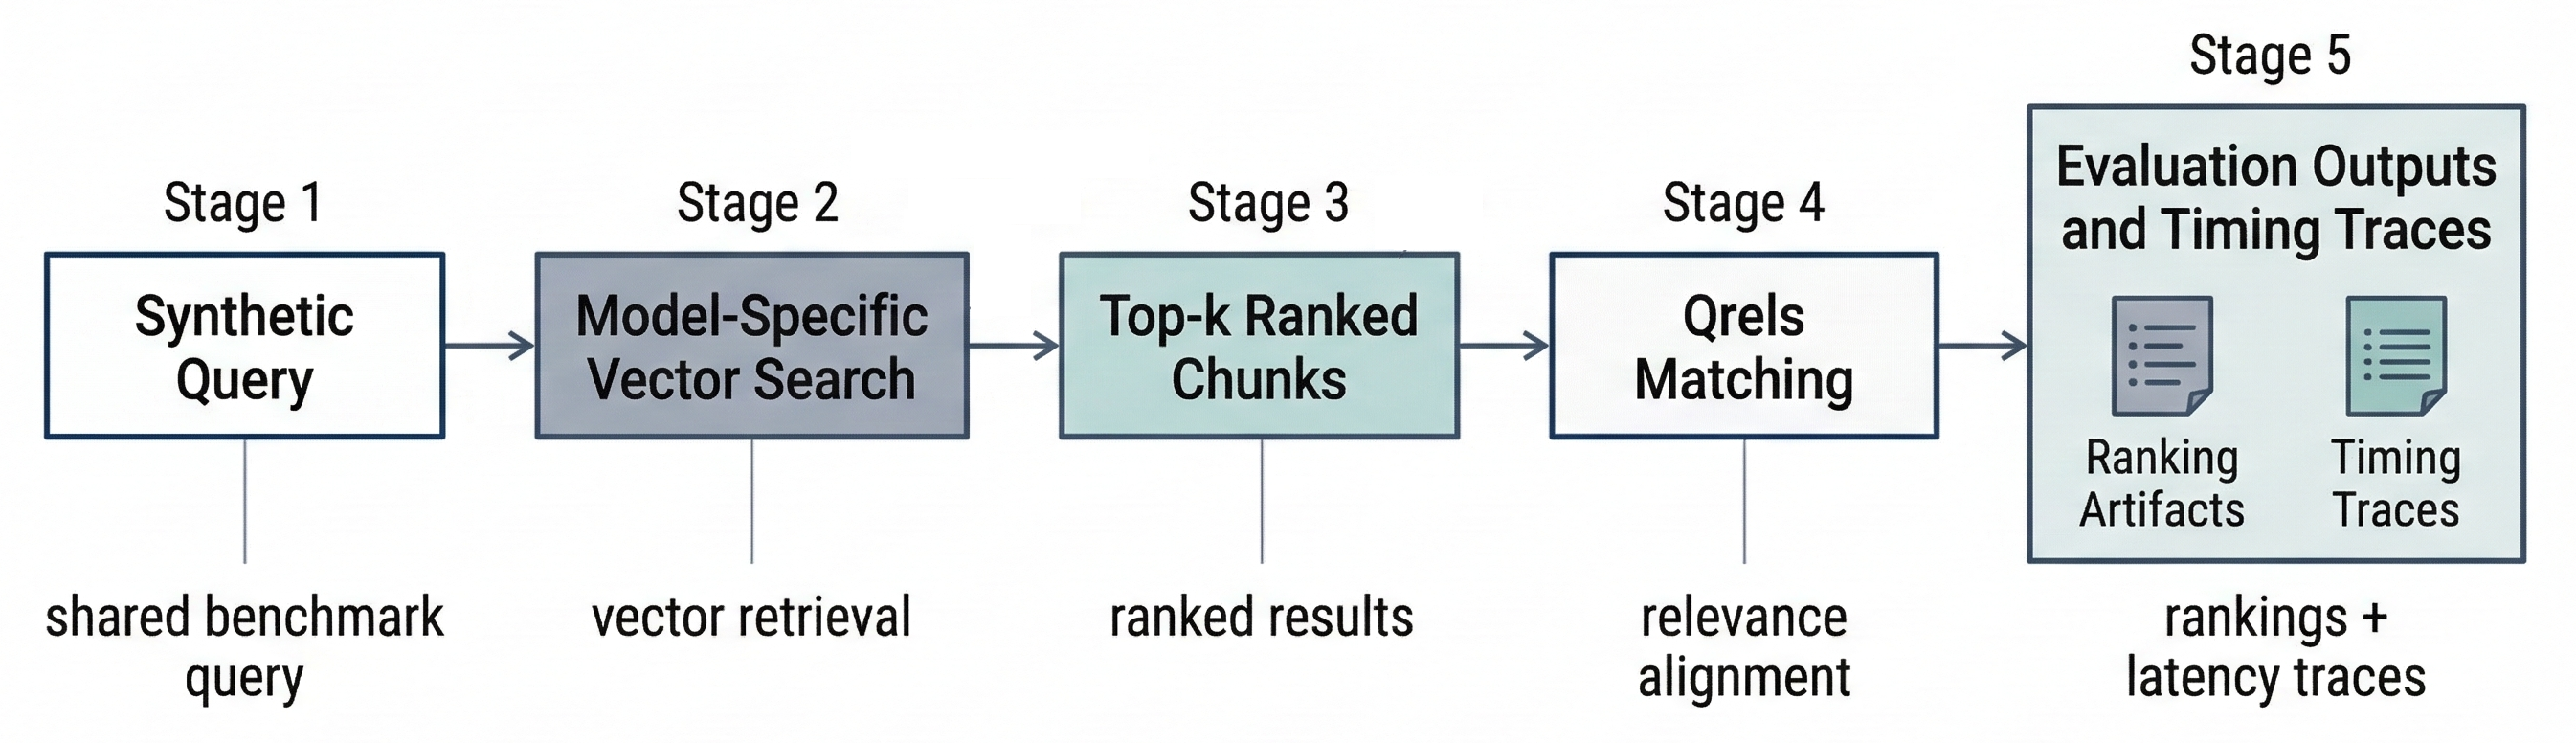
\includegraphics[width=0.95\linewidth]{evaluation_workflow.png}
\caption{Retrieval evaluation workflow from model-specific vector search to evaluation-ready ranking artifacts.}\label{fig:method_retrieval_workflow}
\end{figure}

\subsection{Automated Reporting and Reproducibility}\label{automated-reporting-and-reproducibility}

The final stage transforms raw benchmark outputs into structured reporting artifacts intended for comparative analysis and engineering reuse. As illustrated in Figure~\ref{fig:method_reporting_workflow}, this workflow is organized in two reporting layers whose outputs are summarized in Table~\ref{tbl:method_reporting_outputs}. The first layer operates separately for each dataset or dataset subset. When the objective is to select a suitable embedding model for one available corpus, or for a representative sample drawn from that corpus, the pipeline can terminate at this stage and produce a single benchmark report together with ranking summaries, timing summaries, and dataset-specific visualizations. These per-dataset artifacts preserve the full evaluation trace for one corpus under the shared model roster and provide a self-contained basis for model selection within that local context.

The second layer begins only after one or more dataset-level reports have been completed. This aggregation stage is intended for settings in which the available collection is heterogeneous, for example when documents belong to different topic classes such as finance, law, or administration, or when the corpus spans multiple languages such as English, Turkish, or French. In such cases, separate benchmark reports can be generated for the relevant subsets and then combined into an aggregate comparison package, as shown in Figure~\ref{fig:method_reporting_workflow}. The aggregate report is therefore derived from completed benchmark products rather than from raw retrieval outputs, which enables automatic inspection of how corpus variation affects embedding behavior across multiple evaluation criteria. The concrete experimental configuration and the resulting comparative evidence are presented in Sections~\ref{experiments} and~\ref{results}, respectively.

\begin{table}[t]
\caption{Reporting outputs produced by the proposed benchmarking pipeline.}\label{tbl:method_reporting_outputs}
\centering
\small
\begin{tabular}{@{}>{\raggedright\arraybackslash}p{0.16\linewidth}>{\raggedright\arraybackslash}p{0.36\linewidth}>{\raggedright\arraybackslash}p{0.36\linewidth}@{}}
\toprule
Output level & Artifacts & Purpose \\
\midrule
Dataset level & Benchmark report, ranking summaries, timing summaries, and dataset-specific visualizations & Support model selection for one corpus, one subset, or one representative sample under the shared model set \\
Aggregate level & Cross-dataset comparison report and comparative visual summaries & Consolidate heterogeneous dataset-level outputs into a reusable comparison package for cross-corpus or cross-subset inspection \\
\bottomrule
\end{tabular}
\end{table}

\begin{figure}
\centering
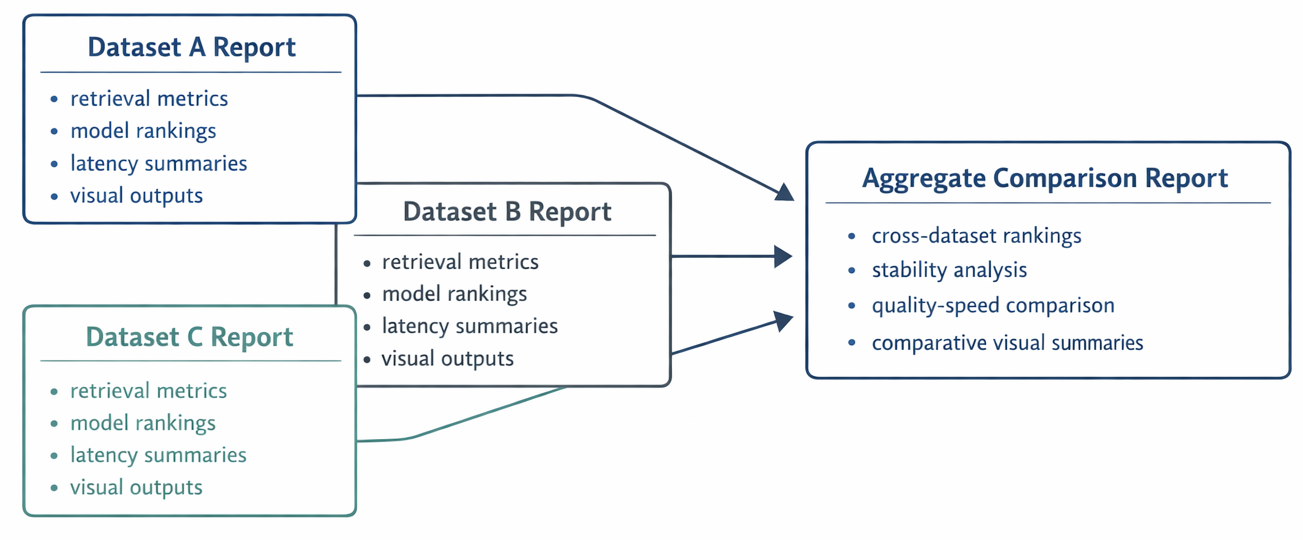
\includegraphics[width=0.95\linewidth]{report_generation.png}
\caption{Reporting flow from dataset-specific benchmark outputs to aggregate comparison artifacts.}\label{fig:method_reporting_workflow}
\end{figure}

The method is designed for reproducibility at both the artifact and workflow levels. Intermediate benchmark resources are materialized as explicit corpus, query, qrels, and report artifacts; model evaluation is performed on isolated vector collections; and reporting outputs are stored as timestamped run products at both dataset and aggregate levels. The implementation of this pipeline is publicly available for inspection and reuse, which supports transparent reconstruction of the benchmarking workflow described in this paper. \citep{GitHub_RagRetrievalBench}

\section{Experiments}\label{experiments}

\subsection{Experimental Snapshot}\label{experimental-snapshot}

This section instantiates the generic benchmarking pipeline described in Section~\ref{method} under one fixed experimental configuration. All experiments reported in this paper were generated within a single internally consistent benchmark snapshot so that dataset preparation, model evaluation, and cross-dataset comparison remain directly comparable. The objective of this setup is to demonstrate the practical use of the proposed pipeline for local embedding-model selection rather than to claim universal superiority for any one model.

The experimental design follows a reusable decision-support pattern. A practitioner first defines one or more local document collections, applies the same preprocessing and benchmark-construction procedure to each collection, and evaluates the same candidate model roster under one shared setup. As shown in Figure~\ref{fig:experiment_snapshot_design}, this process yields repeated dataset-level benchmark outputs for each corpus before any higher-level comparison is attempted. The aggregate comparison stage is then constructed from these completed per-dataset outputs rather than from an alternative evaluation branch. In this paper, the design is instantiated with three corpora and five embedding models.

\begin{figure}
\centering
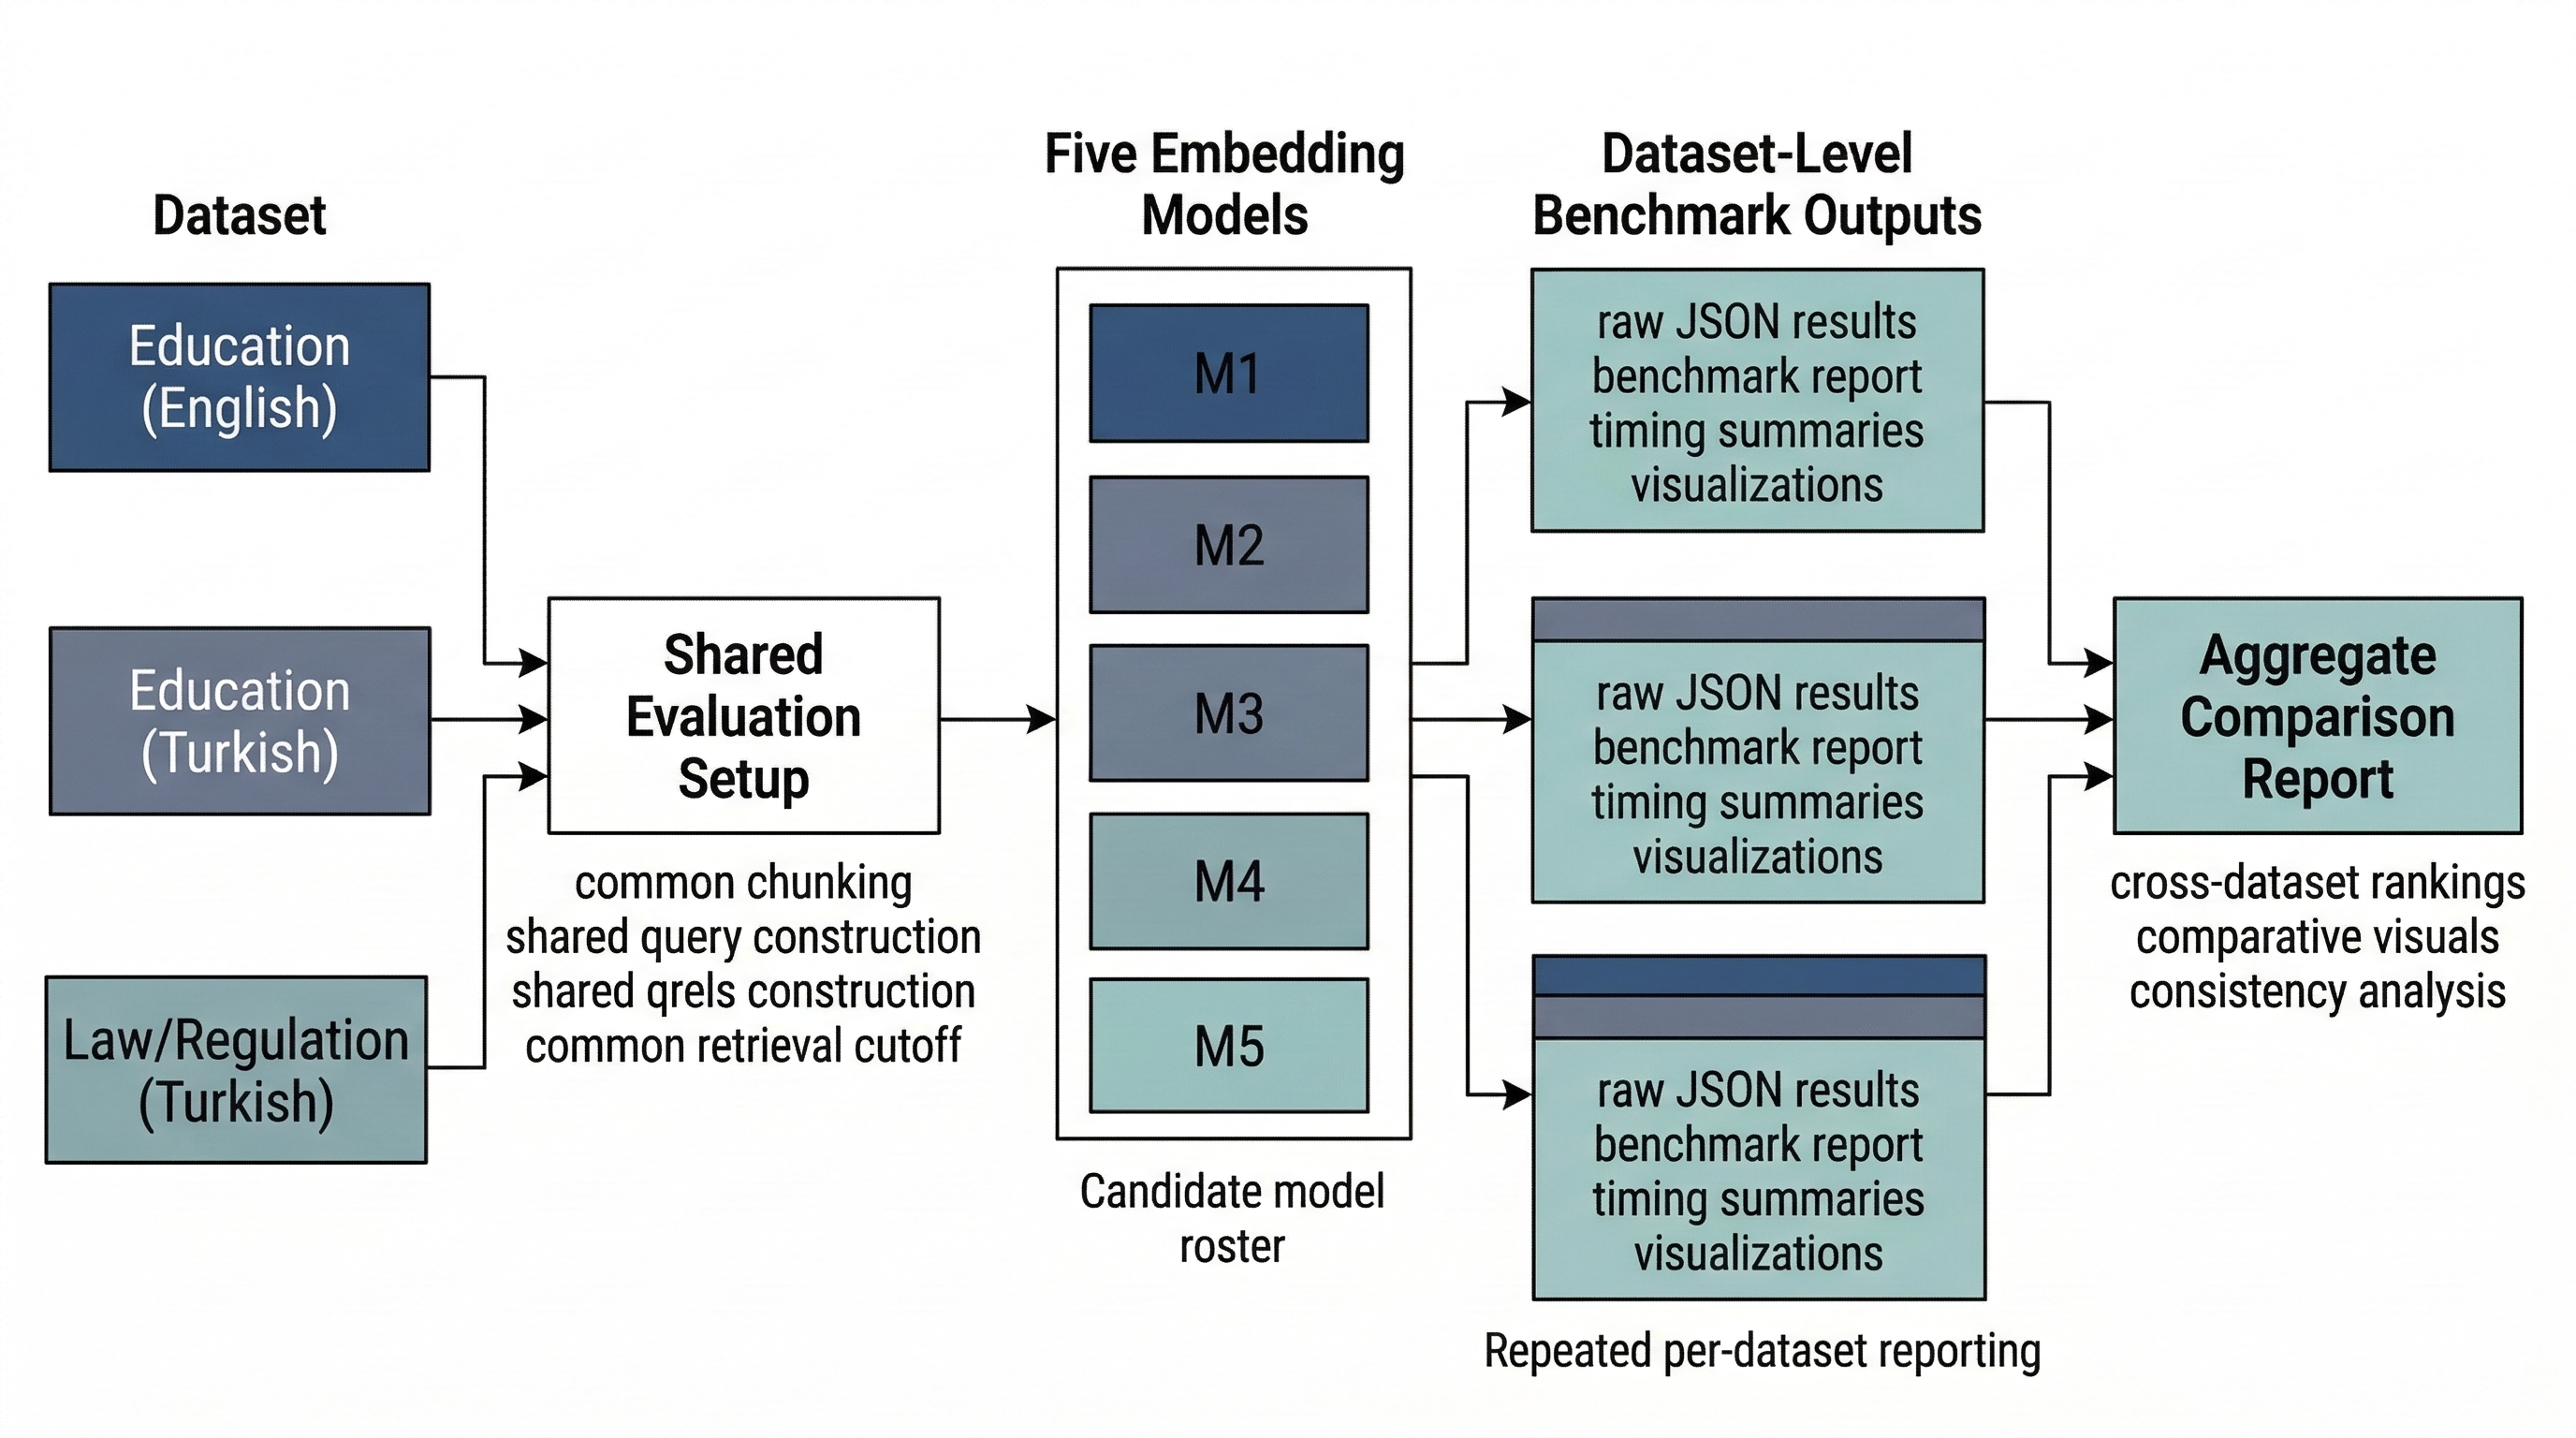
\includegraphics[width=0.95\linewidth]{experimental_design.png}
\caption{Experimental design used to instantiate the proposed benchmarking pipeline in this paper.}\label{fig:experiment_snapshot_design}
\end{figure}

\subsection{Datasets}\label{datasets}

The benchmark covers three local datasets chosen to expose both language variation and domain variation within one controlled setup. Two corpora belong to the education domain and are provided in English and Turkish, whereas the third corpus belongs to the Turkish legal and regulatory domain. For compact reference in the paper, these datasets are denoted as \texttt{education\_eng}, \texttt{education\_tr}, and \texttt{law\_tr}, respectively. This composition allows the same evaluation workflow to be examined across corpora that differ in language, topic, document structure, and corpus scale. Figure~\ref{fig:experiment_dataset_structure} makes this organization explicit by grouping the datasets first by domain and then by language, while also displaying the workload counts associated with each subset. The corresponding quantitative workload summary and source-provenance boundary are reported in Table~\ref{tbl:dataset_statistics_summary} and Table~\ref{tbl:dataset_provenance}, respectively.

Table~\ref{tbl:dataset_statistics_summary} summarizes the same per-dataset counts in tabular form after document ingestion, chunking, synthetic query generation, and qrels construction. The frozen experimental snapshot contains 60 source documents, 1{,}914 chunks, 150 synthetic queries, and 952 positive relevance judgments in total (explicit non-relevant judgments are also stored; see Section~\ref{method}). These counts define the benchmark workload on which the candidate embedding models were evaluated. Taken together, Figure~\ref{fig:experiment_dataset_structure} and Table~\ref{tbl:dataset_statistics_summary} show an important structural characteristic of the benchmark: although \texttt{law\_tr} contains only two source documents, it yields more chunks than either education dataset. The present dataset collection should therefore be read as an intentionally diverse experimental snapshot that combines language, domain, and document-structure variation within one reusable evaluation design. In the present implementation, these source documents were processed from PDF files, but the experimental logic is framed at the document-collection level rather than at one fixed file format.

\begin{table}[t]
\caption{Dataset statistics summary for the frozen experimental snapshot.}\label{tbl:dataset_statistics_summary}
\centering
\begin{tabular}{@{}lrrrr@{}}
\toprule
Dataset & Source documents & Chunks & Queries & Qrels \\
\midrule
education\_eng & 29 & 572 & 50 & 312 \\
education\_tr & 29 & 619 & 50 & 354 \\
law\_tr & 2 & 723 & 50 & 286 \\
Total & 60 & 1914 & 150 & 952 \\
\bottomrule
\end{tabular}
\end{table}

\subsection{Dataset Provenance}\label{dataset-provenance}

Table~\ref{tbl:dataset_provenance} records the provenance boundary of the datasets used in the paper. Its columns summarize the dataset identifier used in this paper, the corresponding language-and-domain category, and the source collection from which the benchmark subset was curated. The education corpora were curated from the TED University regulations and guidelines collection \citep{TED_Regulations}, whereas the law corpus was curated from the BDDK regulations listing \citep{BDDK_Mevzuat}. All source material was retrieved on \texttt{01/01/2026}. The curated benchmark datasets used in this paper are also distributed through the public RagRetrievalBench repository \citep{GitHub_RagRetrievalBench}, which makes the experimental setup directly reusable for follow-up benchmarking studies. Explicit provenance is important because the benchmark is intended as a reusable local evaluation workflow: when the same procedure is applied to a different institutional collection, domain archive, or multilingual document set, the resulting evidence should be interpreted relative to that corpus boundary.

\begin{table}[t]
\caption{Provenance sources for the benchmark datasets used in this paper.}\label{tbl:dataset_provenance}
\centering
\begin{tabular}{@{}>{\raggedright\arraybackslash}p{0.24\linewidth}>{\raggedright\arraybackslash}p{0.26\linewidth}>{\raggedright\arraybackslash}p{0.42\linewidth}@{}}
\toprule
Dataset & Language and domain & Source \\
\midrule
education\_eng & English education & TED University regulations and guidelines \\
education\_tr & Turkish education & TED University regulations and guidelines \\
law\_tr & Turkish law/regulation & BDDK regulations listing \\
\bottomrule
\end{tabular}
\end{table}

The conceptual organization of the benchmark datasets is illustrated in Figure~\ref{fig:experiment_dataset_structure}. This structure is not itself a result; rather, it explains why the present snapshot, together with the workload statistics in Table~\ref{tbl:dataset_statistics_summary}, is suitable for demonstrating both language-sensitive and domain-sensitive use of the benchmarking pipeline.

\begin{figure}
\centering
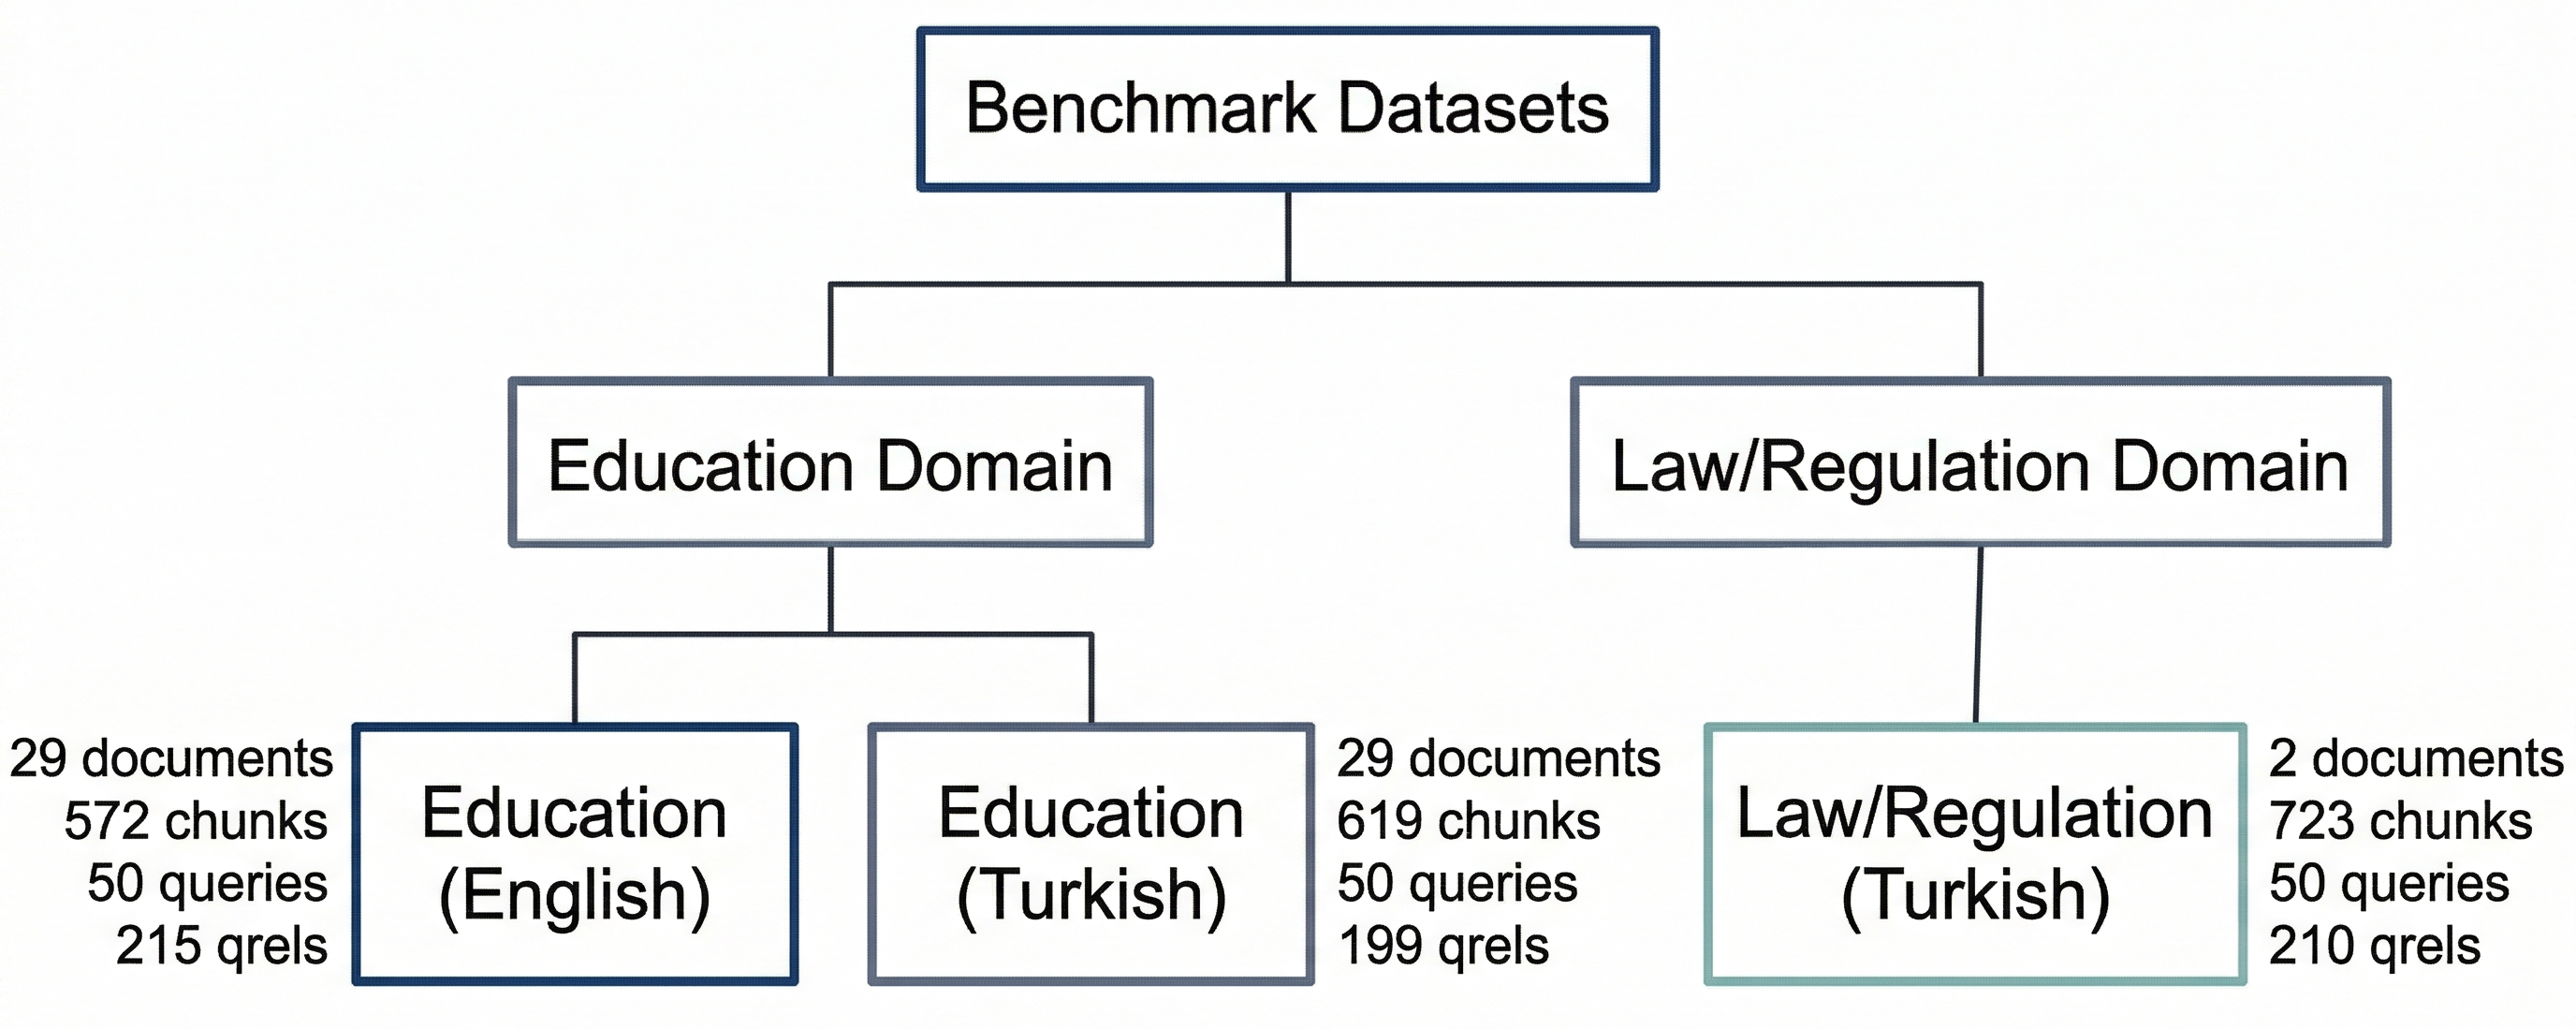
\includegraphics[width=0.95\linewidth]{benchmark_datasets.png}
\caption{Conceptual organization of the benchmark datasets by language and domain, with per-dataset workload counts.}\label{fig:experiment_dataset_structure}
\end{figure}

\subsection{Shared Evaluation Setup}\label{shared-evaluation-setup}

All datasets were processed under the same evaluation configuration so that the main experimental differences arise from corpus characteristics and embedding-model behavior rather than from changes in the benchmark protocol. Retrieval used ChromaDB vector search under its default squared-Euclidean (L2) distance space, with retrieved distances mapped to similarity scores by $1/(1+d)$ for ranking, the common retrieval cutoff was fixed at \texttt{k=10}, chunking used a size of \texttt{1000} characters with \texttt{200} characters of overlap, 50 synthetic queries were generated per dataset, and qrels construction pooled the top-20 candidates retrieved by each of the five models into one model-independent candidate set before LLM judging (Section~\ref{method}). In the pipeline implementation, these experiment-related parameters are stored in a central configuration file, which makes the setup directly accessible and readily adjustable when a practitioner needs to benchmark a different corpus, alternative model roster, or modified operating constraint \citep{ChromaDB_Docs,GitHub_RagRetrievalBench}. This design choice supports the practical aim of the pipeline: the same benchmarking procedure can be adopted as a baseline configuration and then adapted systematically to corpus-specific requirements without changing the overall evaluation logic. Table~\ref{tbl:experiment_workflow_parameters} summarizes the fixed parameter values that define this shared setup across chunking, query construction, index creation, and retrieval evaluation. These values are demonstration-scale defaults rather than tuned optima: 50 queries per dataset, a candidate pool of 20, a chunk size of 1000 characters with 200 of overlap, and a retrieval cutoff of \texttt{k=10} follow common practitioner defaults and the repository's baseline configuration. They are held fixed here so that differences arise from corpus and model rather than from the protocol, and they are exposed as editable configuration; their sensitivity is examined as future work (Section~\ref{conclusion}) rather than claimed to be optimal.

For the present experimental snapshot, synthetic query generation and qrels construction both used the Gemini 2.5 Flash-Lite model. More specifically, the pipeline applies the same LLM family in two roles: first to synthesize a source-language query from each selected seed chunk, and then to act as a binary relevance judge over the retrieved candidate chunks associated with that query. The pipeline supports two operational modes for these LLM-dependent stages. A practitioner may run them through immediate request--response interaction when the benchmark is small or iterative inspection is desired, or may submit them through a batch-processing workflow that separates job submission from result retrieval and can reduce the total cost of larger benchmark runs. This dual execution design improves operational flexibility because the same benchmark logic can be retained while the execution mode is adapted to dataset size, budget, or turnaround constraints \citep{GitHub_RagRetrievalBench}.

\begin{table}[t]
\caption{Fixed workflow parameters used in the shared experimental configuration.}\label{tbl:experiment_workflow_parameters}
\centering
\small
\begin{tabular}{@{}>{\raggedright\arraybackslash}p{0.24\linewidth}>{\raggedright\arraybackslash}p{0.13\linewidth}>{\raggedright\arraybackslash}p{0.51\linewidth}@{}}
\toprule
Parameter & Value & Role in the workflow \\
\midrule
Chunk size & 1000 & Determines the maximum character length of each corpus segment before embedding \\
Chunk overlap & 200 & Preserves continuity between adjacent chunks and reduces boundary-induced information loss \\
Queries per dataset & 50 & Fixes the size of the synthetic evaluation set generated for each corpus \\
Chunks per query seed & 1 & Anchors each generated query to one sampled source chunk during query construction \\
Candidate pool size & 20 & Limits the number of retrieved candidates examined during relevance construction \\
Document batch size & 32 & Controls batched embedding throughput during vector collection construction \\
Collection reinitialization & True & Rebuilds vector collections so each benchmark run starts from a controlled index state \\
Shared retrieval cutoff & 10 & Fixes the number of ranked chunks returned per query during retrieval evaluation \\
\bottomrule
\end{tabular}
\end{table}

Table~\ref{tbl:experiment_embedding_models} lists the embedding model roster used in the experimental configuration. The table identifies each model, its embedding dimension, and its role within the benchmarked roster. This model family was selected because the Sentence Transformers project provides openly available and widely adopted embedding models together with stable documentation and reproducible usage patterns for semantic search applications \citep{SentenceTransformers_Website}. In addition, the five models benchmarked in this paper were selected from among the most downloaded models listed in the Sentence Transformers Hugging Face repository, which makes them representative of models that practitioners are likely to consider first when assembling an open embedding baseline \citep{SentenceTransformers_HF_Repo,HuggingFace_SentenceTransformers}. The purpose of the present setup is not to claim that the sentence-transformer family exhausts all relevant embedding choices; rather, it is to demonstrate that the proposed pipeline can evaluate a realistic candidate set under controlled conditions using models that are directly accessible to practitioners and straightforward to reproduce. Because the pipeline is implemented as an open and configurable workflow, the same procedure can be extended to embedding models from other providers when a different deployment requirement or procurement constraint must be studied. For the practical objective of this paper, however, the selected open-weight models provide a sufficient and reproducible test bed for demonstrating the effectiveness of the benchmarking pipeline itself.

\begin{table}[t]
\caption{Embedding model roster used in the experimental configuration.}\label{tbl:experiment_embedding_models}
\centering
\small
\begin{tabular}{@{}>{\raggedright\arraybackslash}p{0.08\linewidth}>{\raggedright\arraybackslash}p{0.44\linewidth}>{\raggedright\arraybackslash}p{0.12\linewidth}>{\raggedright\arraybackslash}p{0.26\linewidth}@{}}
\toprule
ID & Model & Dimension & Role in the benchmark \\
\midrule
M1 & sentence-transformers/all-MiniLM-L6-v2 & 384 & English-trained MiniLM; lightweight efficiency baseline \\
M2 & sentence-transformers/all-mpnet-base-v2 & 768 & English-trained MPNet; higher-capacity English-oriented model \\
M3 & sentence-transformers/paraphrase-multilingual-MiniLM-L12-v2 & 384 & Multilingual (paraphrase) MiniLM; compact cross-language model \\
M4 & sentence-transformers/all-MiniLM-L12-v2 & 384 & English-trained MiniLM; deeper L12 variant \\
M5 & sentence-transformers/paraphrase-multilingual-mpnet-base-v2 & 768 & Multilingual (paraphrase) MPNet; higher-capacity cross-language model \\
\bottomrule
\end{tabular}
\end{table}

Throughout the paper, \emph{English-oriented} (used interchangeably with monolingual) is shorthand for the \texttt{all-MiniLM} and \texttt{all-mpnet} models, which are trained predominantly on English data, while \emph{multilingual} denotes the \texttt{paraphrase-multilingual} models, which are trained on many languages. These labels describe the intended training regime and are used for discussion; they are not strict claims about tokenizer coverage or guaranteed per-language quality.

To preserve comparability across datasets, the experiments held constant the metric definitions and retrieval cutoff, the embedding model roster, the candidate pool size used during qrels construction, the chunking parameters summarized in Table~\ref{tbl:experiment_workflow_parameters}, and the reporting pipeline. The intentionally varying factors were corpus language, domain, corpus size, and document composition. This separation between fixed and varying factors provides a practical guideline for external reuse: a practitioner who wishes to benchmark a different corpus can keep the evaluation frame fixed while substituting a new dataset collection and, if needed, a different candidate model list.

\subsection{Reproducibility Conditions}\label{reproducibility-conditions}

Table~\ref{tbl:reproducibility} summarizes the software, data-processing, and measurement conditions required to reproduce the benchmark; library versions are pinned in the public repository \citep{GitHub_RagRetrievalBench}. Seed-chunk sampling uses a fixed random seed, and each run records an environment snapshot (Python and library versions, device) in its raw-result JSON, so the reported snapshot is reproducible from the released corpus, queries, and qrels. One condition remains a genuine limitation: the reported runs were executed on CPU without a controlled hardware matrix, so the timing measurements should be read as relative, same-machine comparisons between models rather than as absolute, machine-transferable latencies.

\begin{table}[t]
\caption{Reproducibility conditions for the benchmark snapshot.}\label{tbl:reproducibility}
\centering
\small
\begin{tabular}{@{}>{\raggedright\arraybackslash}p{0.30\linewidth}>{\raggedright\arraybackslash}p{0.62\linewidth}@{}}
\toprule
Component & Setting \\
\midrule
Language runtime & Python 3.10 (\texttt{ragbenchmark} conda environment) \\
Vector store & ChromaDB 1.0.7 (persistent client), default squared-Euclidean (L2) space; similarity $1/(1+d)$ \\
Embeddings & Sentence-Transformers 4.1.0 (PyTorch 2.7.0), default non-normalized encoding, batch size 32 \\
Text extraction & PyMuPDF 1.26.0 page text with NFC Unicode normalization \\
Chunking & LangChain recursive character splitter, size 1000, overlap 200 \\
Retrieval evaluation & Sentence-Transformers \texttt{InformationRetrievalEvaluator}, cutoff $k=10$ \\
Query generation and judging & Gemini 2.5 Flash-Lite, temperature 0.1, in batch and interactive modes \\
Candidate pool & Model-independent union of the top-20 chunks retrieved by all five models, LLM-judged with stored positive and negative labels; a single-model (\texttt{M5}-only) variant is compared in Section~\ref{results} \\
Seed policy & Fixed random seed (42) for seed-chunk sampling, so the reported snapshot is reproducible \\
Timing scope & Query latency $=$ query embedding $+$ vector search (local only, measured cold, no LLM or network); embedding time $=$ batched corpus embedding and insertion \\
Hardware / OS / device & Environment snapshot (Python and library versions, device) recorded in each raw-result JSON; the reported runs used CPU, so timing is single-machine and should be read as relative \\
Released artifacts & Corpus, queries, qrels, raw-result JSON, and reports in the public repository \citep{GitHub_RagRetrievalBench} \\
\bottomrule
\end{tabular}
\end{table}

\subsection{Report Outputs and Utility}\label{report-outputs-and-utility}

The reporting outputs generated in these experiments follow the two-layer reporting design described in Section~\ref{automated-reporting-and-reproducibility}, Figure~\ref{fig:method_reporting_workflow}, and Table~\ref{tbl:method_reporting_outputs}. For each dataset run, the pipeline first materializes the evaluation state as a machine-readable raw-result JSON artifact. These stored results preserve the essential benchmark record, including the applied configuration, corpus and query statistics, qrels characteristics, per-model retrieval scores, and timing measurements. This design is important for practical reuse because the underlying experimental evidence remains available for later verification, archival reference, re-analysis, or downstream comparison without requiring the retrieval workflow to be executed again.

The human-readable benchmark reports are then generated from these stored JSON results rather than from transient console output. At the dataset level, the pipeline produces a benchmark report together with ranking summaries, timing summaries, and visualization assets covering metric profiles, ranking comparisons, consistency patterns, and timing behavior. This separation between raw-result storage and report generation makes the setup easier to reuse in practice: a practitioner can preserve the original benchmark evidence, regenerate presentation-oriented summaries when needed, and inspect one dataset or one representative subset as a self-contained decision-support case.

When multiple dataset runs are available, the aggregate reporting stage loads the dataset-level JSON artifacts and constructs a cross-dataset comparison report with comparative visual summaries. In the present paper, this second reporting layer provides the experimental basis for comparing embedding behavior across language- and domain-differentiated subsets under one shared setup. Within the experimental section, these reporting products are operational outputs of the benchmark procedure rather than findings in themselves. The substantive comparative evidence derived from them is presented separately in Section~\ref{results}.

\section{Results}\label{results}

This section reports the evidence produced by the proposed benchmarking pipeline under the fixed experimental setup described in Section~\ref{experiments}. The purpose of the reported results is practical model selection for local corpora rather than universal leaderboard comparison. Because the pipeline generates full benchmark reports automatically and dynamically, only a selected subset of the most decision-relevant tables and figures is included here. The full automatically generated reports and supporting artifacts are available through the public repository for interested readers. \citep{GitHub_RagRetrievalBench}

\subsection{Cross-Dataset Headline Findings}\label{cross-dataset-headline-findings}

The fixed three-dataset snapshot yields three immediate findings. First, Table~\ref{tbl:cross_dataset_consistency_summary} shows that the multilingual mpnet model (\texttt{M5}) is the strongest overall candidate by average rank and mean \texttt{MAP@10}. Second, Table~\ref{tbl:dataset_result_summary} shows that retrieval difficulty is dataset-dependent: \texttt{education\_eng} is the easiest benchmark in this paper, whereas \texttt{law\_tr} is the hardest. Third, Figure~\ref{fig:results_cross_dataset_performance} shows that the English benchmark is more tightly clustered at a high absolute score level, while the Turkish benchmarks separate more strongly by language and domain. Taken together, these shared-protocol artifacts show that the pipeline can turn heterogeneous local corpora into one directly comparable decision-support view, which is the paper's main answer to RQ1. The aggregate diagnostics in Table~\ref{tbl:cross_dataset_consistency_summary} extend that answer by showing that the workflow also produces robustness evidence, not only point estimates: the same benchmark can identify models that are strong on average, models that degrade sharply under language or domain shift, and models whose behavior is comparatively stable across the full metric set.

\begin{table}[t]
\caption{Dataset-level performance summary for the fixed experimental snapshot.}\label{tbl:dataset_result_summary}
\centering
\begin{tabular}{@{}l>{\raggedright\arraybackslash}p{0.33\linewidth}rr@{}}
\toprule
Dataset & Best model & Top MAP@10 & Mean MAP@10 \\
\midrule
education\_eng & M4 & 0.6121 & 0.5737 \\
education\_tr & M5 & 0.5508 & 0.2912 \\
law\_tr & M5 & 0.3659 & 0.2065 \\
\bottomrule
\end{tabular}
\end{table}

\begin{table}[t]
\caption{Cross-dataset aggregate ranking and consistency diagnostics for the benchmarked embedding models.}\label{tbl:cross_dataset_consistency_summary}
\centering
\small
\begin{tabular}{@{}lrrrrrr@{}}
\toprule
Model & Avg Rank & Mean MAP@10 & All-metric CV & Worst drop & Score range & Wins \\
\midrule
M5 & 2.00 & 0.4857 & 0.357 & 0.743 & 0.728 & 2 \\
M4 & 2.33 & 0.3299 & 0.608 & 0.910 & 0.910 & 1 \\
M3 & 3.00 & 0.4281 & 0.399 & 0.794 & 0.762 & 0 \\
M1 & 3.67 & 0.2789 & 0.741 & 0.927 & 0.908 & 0 \\
M2 & 4.00 & 0.2631 & 0.796 & 0.932 & 0.932 & 0 \\
\bottomrule
\end{tabular}
\end{table}

Table~\ref{tbl:cross_dataset_consistency_summary} connects the aggregate ranking to the paper's language and domain claims. Average rank and mean \texttt{MAP@10} identify strong aggregate performers, while all-metric CV, worst drop, and score range show how stable each model is across the six retrieval metrics and three dataset conditions. This supports RQ2 and RQ3 because the largest drops occur when model behavior interacts with corpus language and domain: the English-oriented models remain competitive on \texttt{education\_eng} but become much less stable across the Turkish conditions, whereas \texttt{M5} combines the best average rank with the smallest consistency penalty in this snapshot.

\begin{figure}
\centering
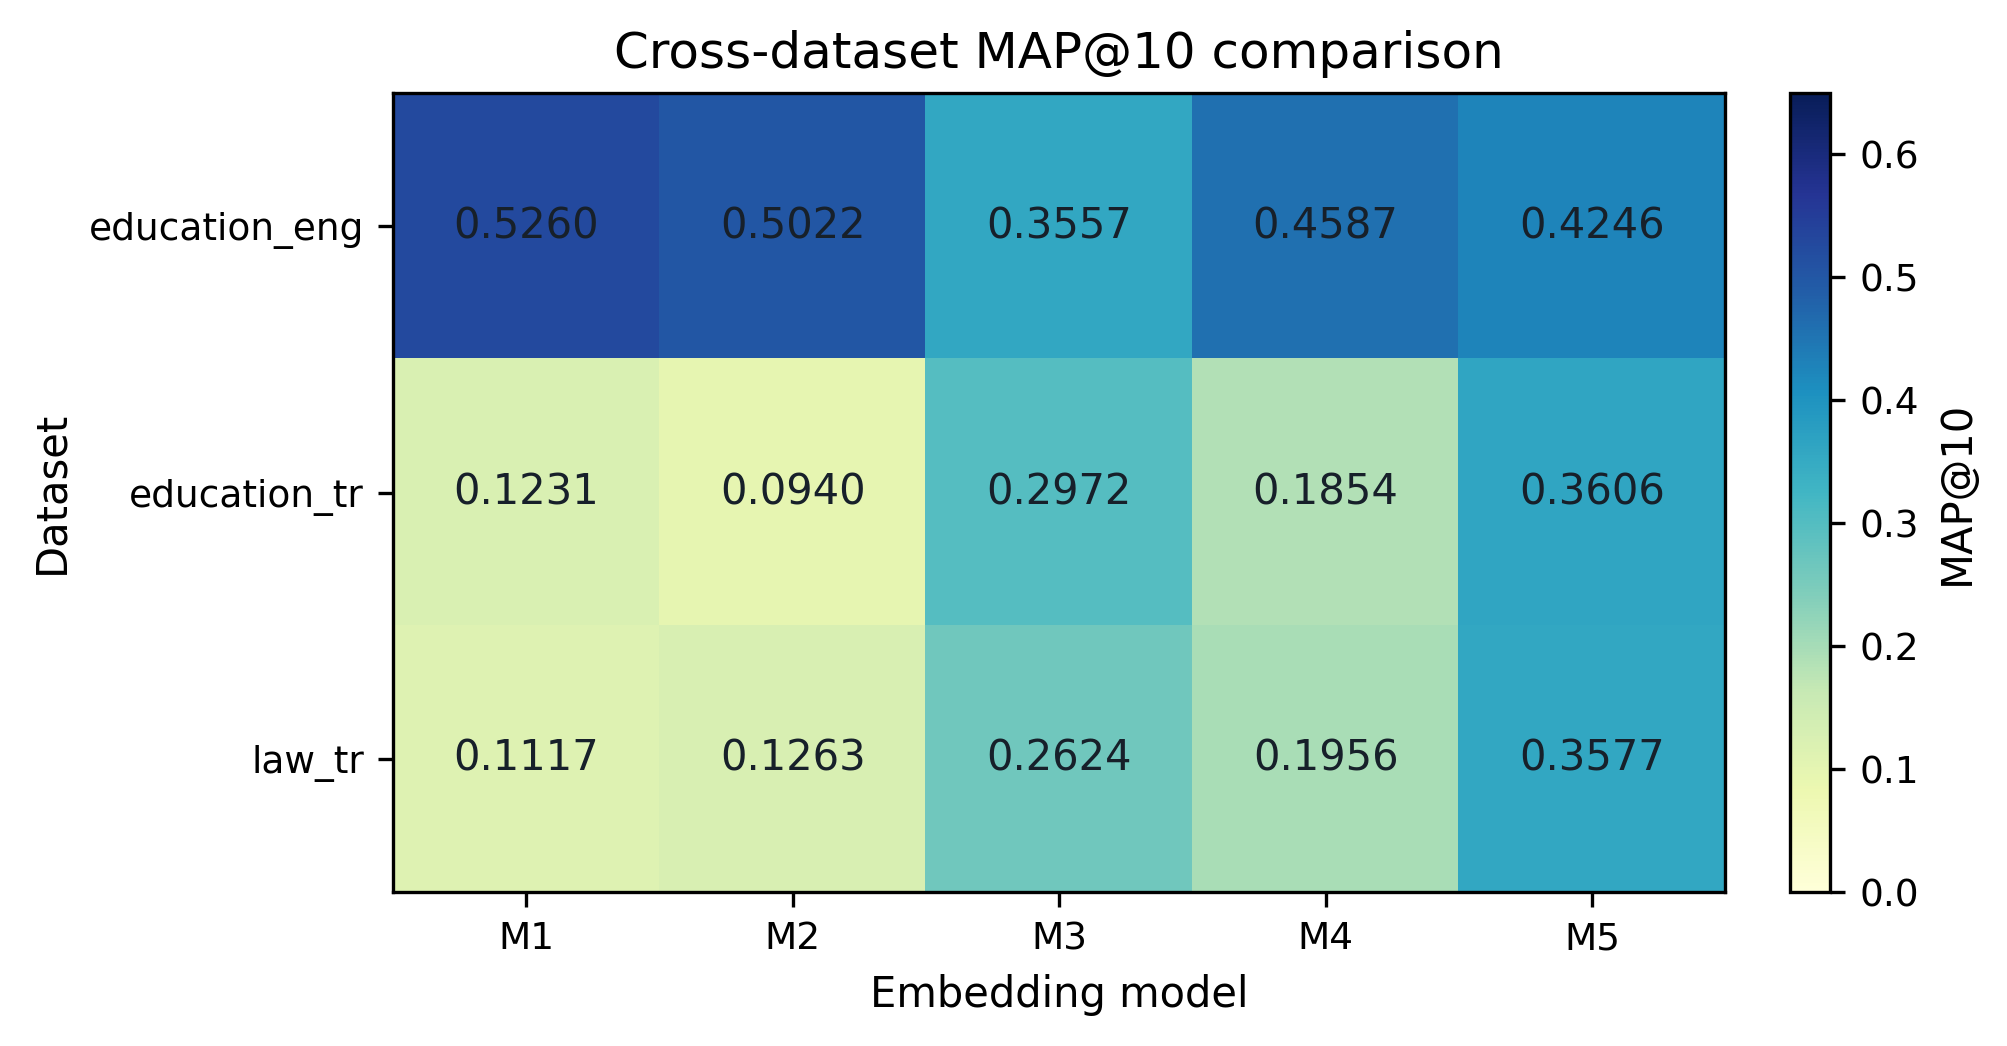
\includegraphics[width=0.92\linewidth]{results_cross_dataset_performance.png}
\caption{Cross-dataset \texttt{MAP@10} comparison for the five benchmarked embedding models.}\label{fig:results_cross_dataset_performance}
\end{figure}

\subsection{Dataset-Level Results: education\_eng}\label{results-education-eng}

The English education subset produces the strongest retrieval scores in the present paper. Table~\ref{tbl:education_eng_metrics} shows that three monolingual models (\texttt{M4}, \texttt{M2}, and \texttt{M1}) cluster closely at the top of the ranking, with \texttt{M4} reaching the highest \texttt{MAP@10} at 0.6121, followed almost immediately by \texttt{M2} at 0.6074 and \texttt{M1} at 0.6067. Figure~\ref{fig:results_education_eng_model_comparison} reinforces this pattern by showing that the top three models remain tightly grouped across the full metric profile rather than separating on only one score.

Table~\ref{tbl:education_eng_timing}, however, shows that these near-tied quality results come with different operational costs: \texttt{M1} has the lowest query latency at 28.10 ms/query, \texttt{M4} remains close at 32.36 ms/query, and \texttt{M2} is much slower at 58.41 ms/query. For English education corpora, the benchmark therefore narrows the practical shortlist to \texttt{M4}, \texttt{M1}, and \texttt{M2}: \texttt{M4} is the strongest quality-first choice, \texttt{M1} is the latency-first choice, and \texttt{M2} is mainly defensible when its near-top retrieval quality matters more than its higher cost.

\begin{table}[t]
\caption{Retrieval metrics for the \texttt{education\_eng} dataset.}\label{tbl:education_eng_metrics}
\centering
\small
\begin{tabular}{@{}lrrrrrr@{}}
\toprule
Model & MAP@10 & Recall@10 & Precision@10 & NDCG@10 & MRR@10 & Success@10 \\
\midrule
M1 & 0.6067 & 0.7984 & 0.300 & 0.7227 & 0.8147 & 0.98 \\
M2 & 0.6074 & 0.7654 & 0.292 & 0.7163 & 0.8216 & 1.00 \\
M3 & 0.5020 & 0.6838 & 0.270 & 0.6146 & 0.7060 & 0.92 \\
M4 & 0.6121 & 0.8183 & 0.316 & 0.7345 & 0.8260 & 1.00 \\
M5 & 0.5404 & 0.7666 & 0.310 & 0.6703 & 0.7747 & 0.98 \\
\bottomrule
\end{tabular}
\end{table}

\begin{table}[t]
\caption{Timing summary for the \texttt{education\_eng} dataset.}\label{tbl:education_eng_timing}
\centering
\small
\begin{tabular}{@{}lrrr@{}}
\toprule
Model & Chunks/s & Avg ms/chunk & Query latency (ms/query) \\
\midrule
M1 & 57.1 & 17.51 & 28.10 \\
M2 & 8.6 & 115.92 & 58.41 \\
M3 & 48.2 & 20.73 & 35.30 \\
M4 & 47.3 & 21.14 & 32.36 \\
M5 & 15.1 & 66.02 & 63.54 \\
\bottomrule
\end{tabular}
\end{table}

\begin{figure}
\centering
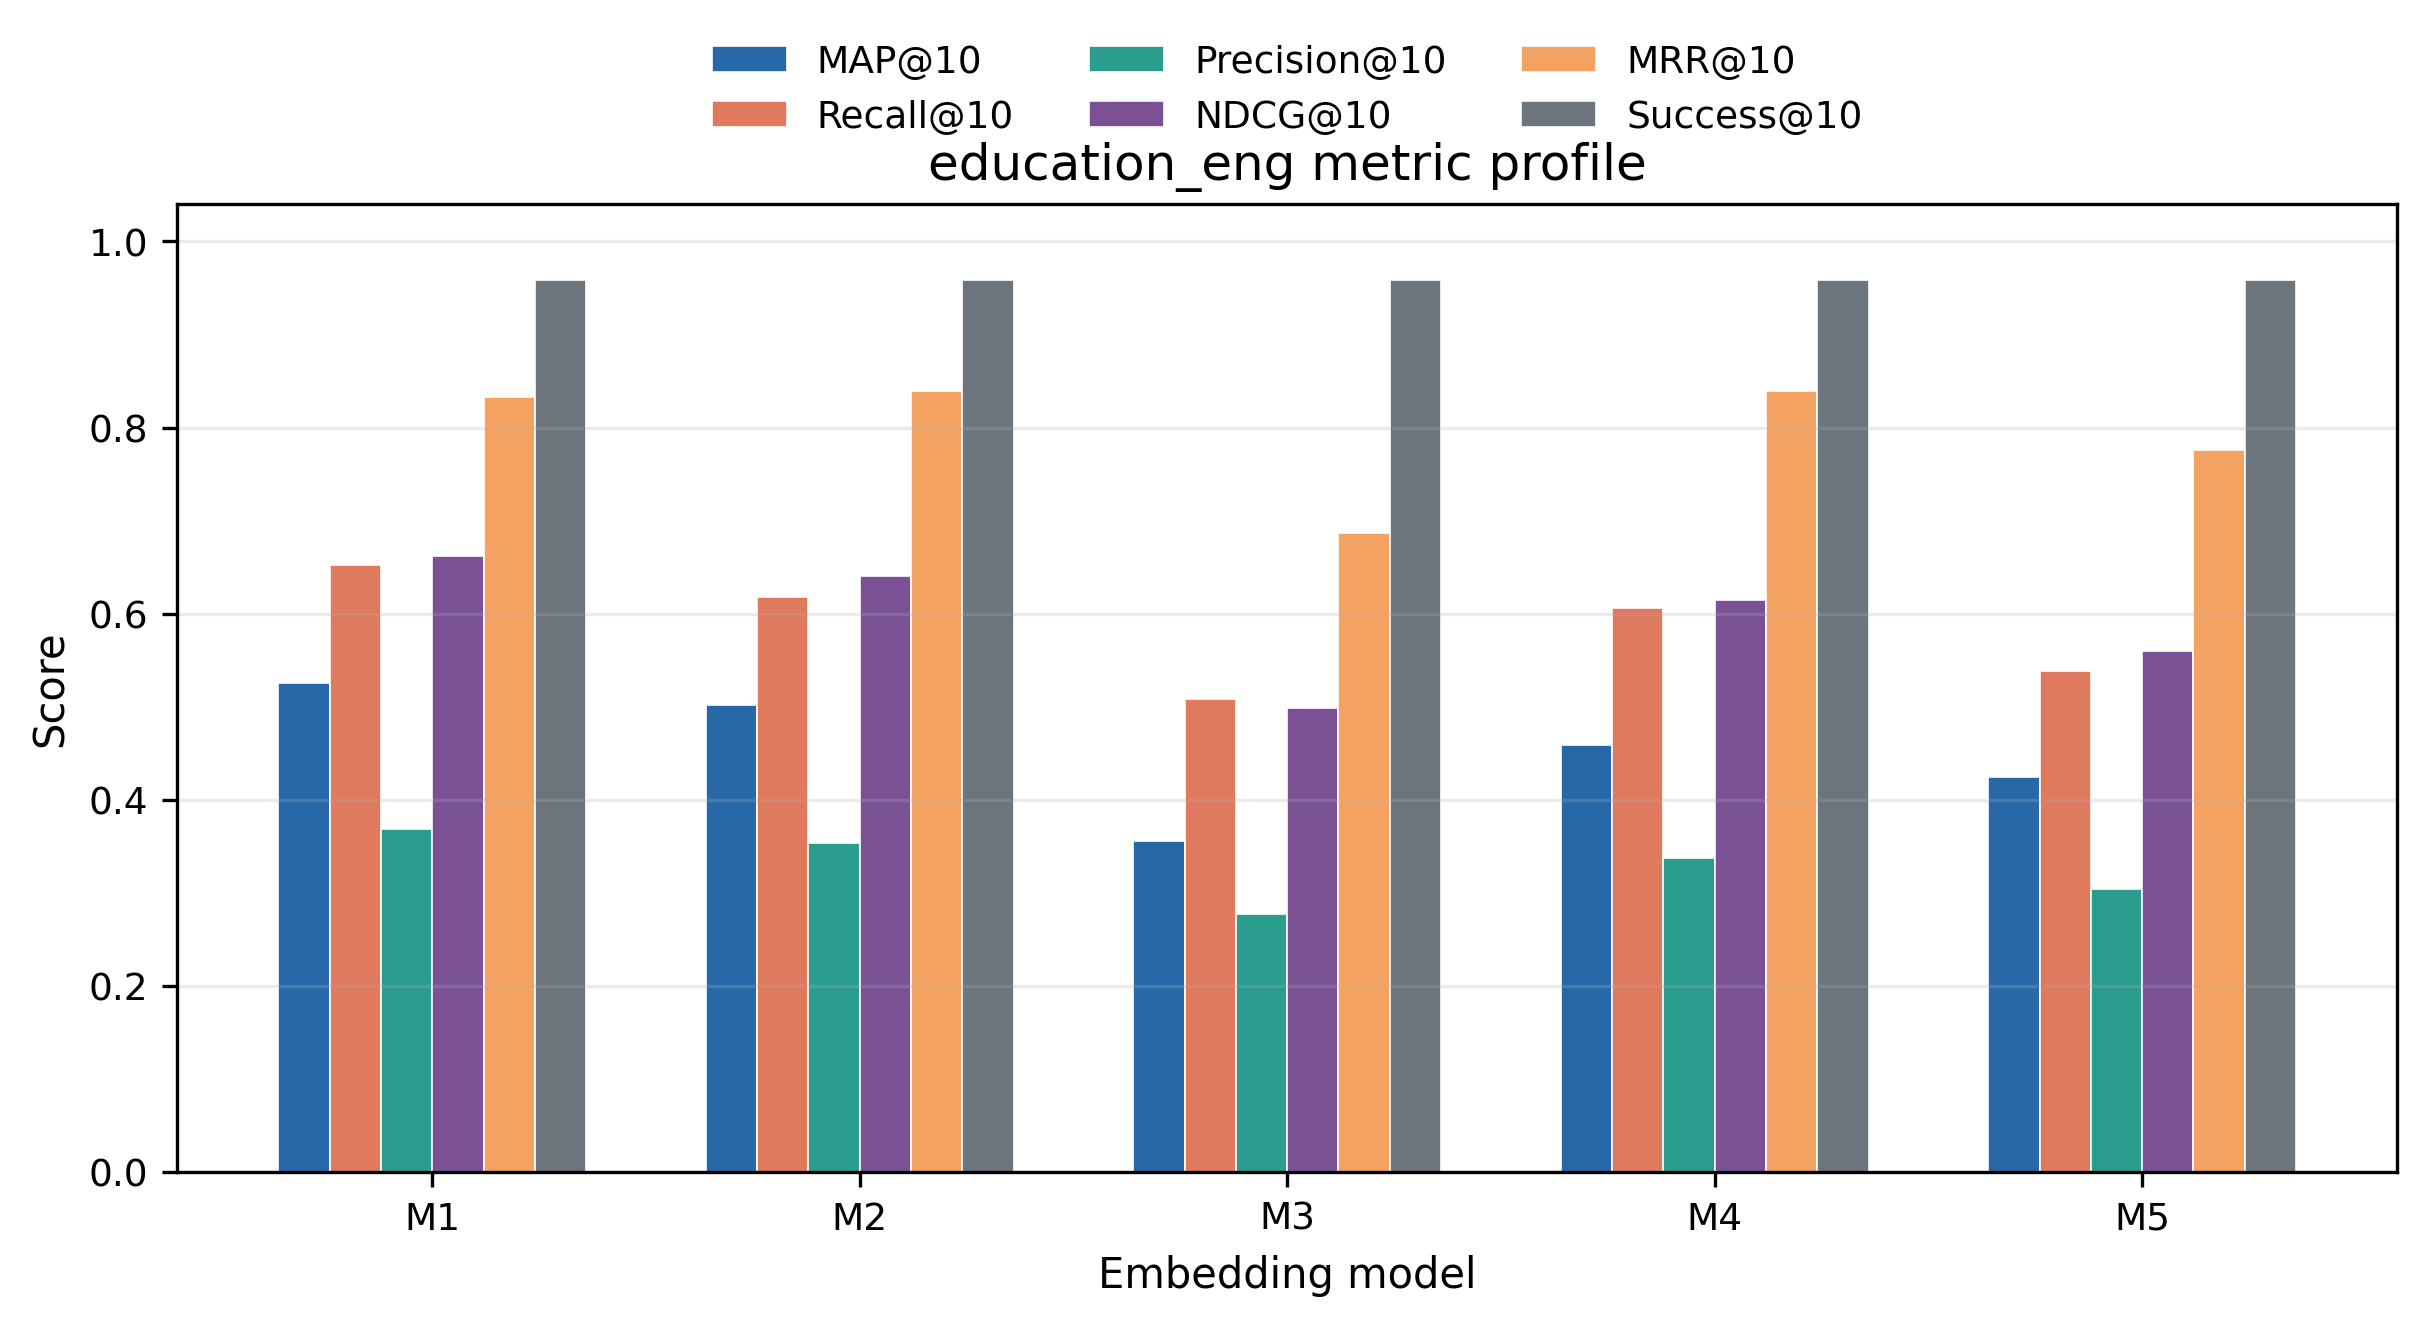
\includegraphics[width=0.92\linewidth]{results_education_eng_model_comparison.png}
\caption{Representative per-dataset metric profile generated automatically for the \texttt{education\_eng} benchmark.}\label{fig:results_education_eng_model_comparison}
\end{figure}

\subsection{Dataset-Level Results: education\_tr}\label{results-education-tr}

The Turkish education subset reverses the preferred model family. As shown in Table~\ref{tbl:education_tr_metrics}, the multilingual models \texttt{M5} and \texttt{M3} clearly separate from the three monolingual alternatives across all six retrieval metrics, with \texttt{M5} reaching 0.5508 \texttt{MAP@10}, \texttt{M3} reaching 0.4876, and the next-best monolingual model \texttt{M4} reaching only 0.1915. Figure~\ref{fig:results_education_tr_model_comparison} makes this sharper ranking visible by showing a clean multilingual-versus-monolingual split across the full metric profile.

Table~\ref{tbl:education_tr_timing} shows that the quality advantage is obtained at different costs: \texttt{M3} remains relatively close to the lightweight models at 34.84 ms/query, whereas the higher-capacity \texttt{M5} rises to 58.75 ms/query. For Turkish education corpora, the pipeline therefore reduces the practical candidate set to \texttt{M5} and \texttt{M3}: \texttt{M5} is preferred when retrieval effectiveness dominates, while \texttt{M3} is the lower-latency compromise.

\begin{table}[t]
\caption{Retrieval metrics for the \texttt{education\_tr} dataset.}\label{tbl:education_tr_metrics}
\centering
\small
\begin{tabular}{@{}lrrrrrr@{}}
\toprule
Model & MAP@10 & Recall@10 & Precision@10 & NDCG@10 & MRR@10 & Success@10 \\
\midrule
M1 & 0.1371 & 0.2397 & 0.088 & 0.2061 & 0.3019 & 0.50 \\
M2 & 0.0891 & 0.2031 & 0.068 & 0.1473 & 0.1976 & 0.46 \\
M3 & 0.4876 & 0.6702 & 0.240 & 0.6137 & 0.7585 & 0.96 \\
M4 & 0.1915 & 0.2768 & 0.090 & 0.2647 & 0.4013 & 0.62 \\
M5 & 0.5508 & 0.7413 & 0.290 & 0.6715 & 0.7830 & 0.98 \\
\bottomrule
\end{tabular}
\end{table}

\begin{table}[t]
\caption{Timing summary for the \texttt{education\_tr} dataset.}\label{tbl:education_tr_timing}
\centering
\small
\begin{tabular}{@{}lrrr@{}}
\toprule
Model & Chunks/s & Avg ms/chunk & Query latency (ms/query) \\
\midrule
M1 & 48.0 & 20.85 & 29.36 \\
M2 & 3.9 & 259.30 & 75.98 \\
M3 & 45.3 & 22.09 & 34.84 \\
M4 & 43.8 & 22.83 & 42.60 \\
M5 & 14.3 & 70.05 & 58.75 \\
\bottomrule
\end{tabular}
\end{table}

\begin{figure}
\centering
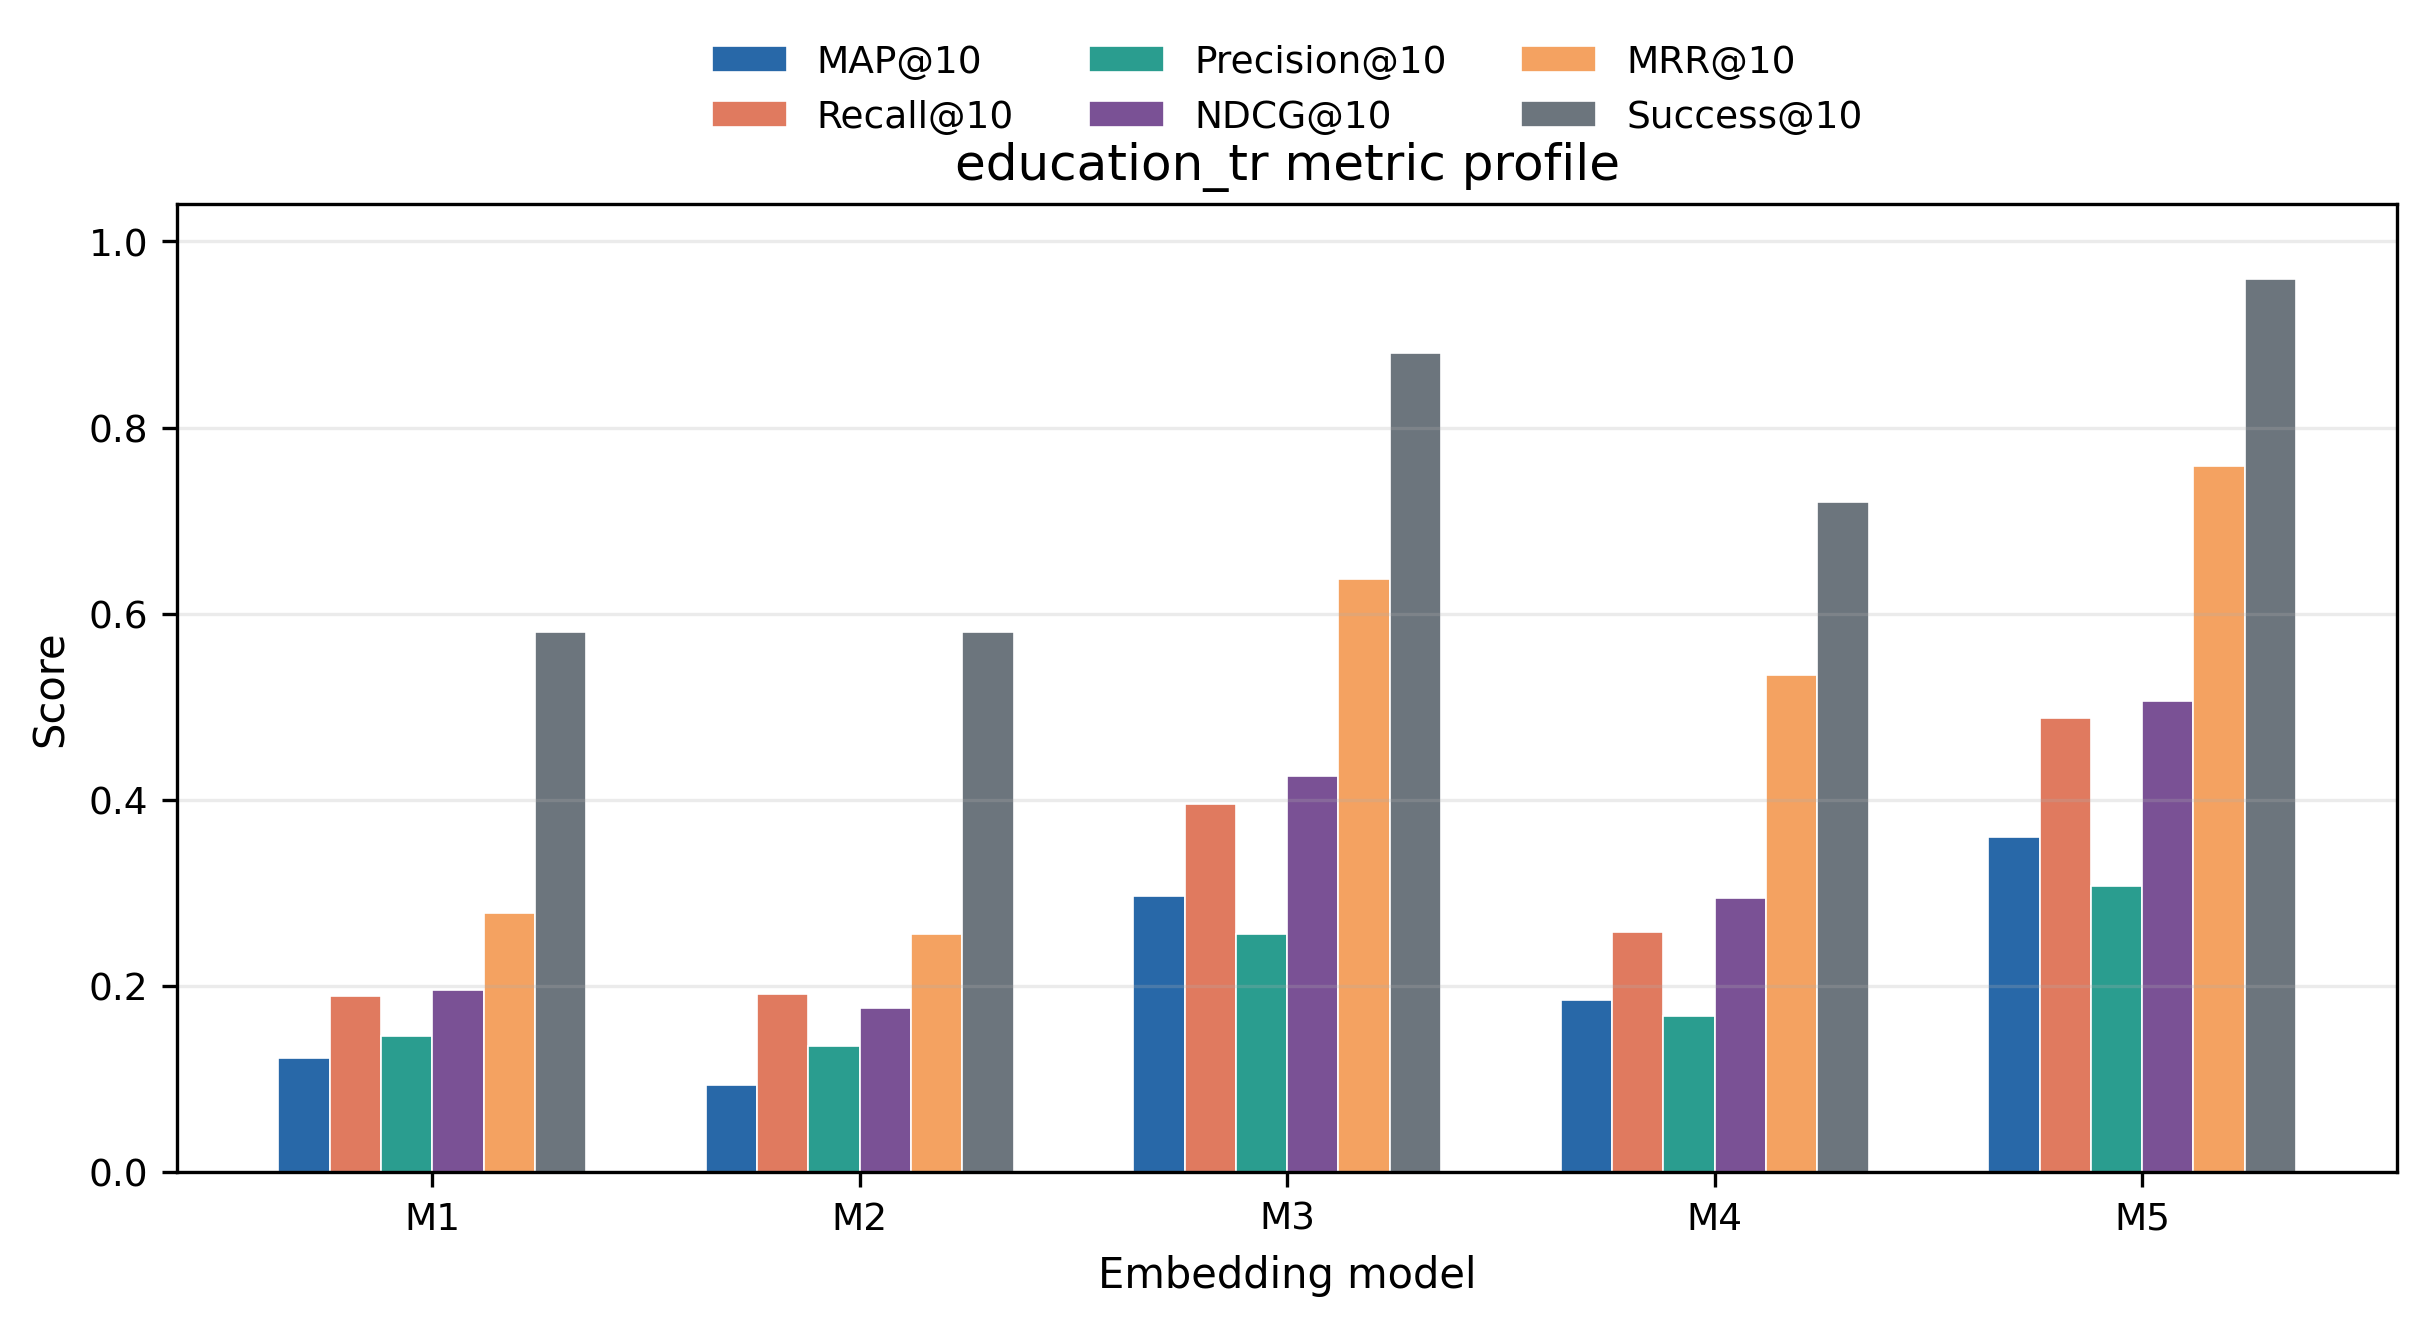
\includegraphics[width=0.92\linewidth]{results_education_tr_model_comparison.png}
\caption{Representative per-dataset metric profile generated automatically for the \texttt{education\_tr} benchmark.}\label{fig:results_education_tr_model_comparison}
\end{figure}

\subsection{Dataset-Level Results: law\_tr}\label{results-law-tr}

The Turkish law/regulation subset is the most difficult benchmark in the fixed snapshot, yet it preserves the same top-two ordering observed in \texttt{education\_tr}. Table~\ref{tbl:law_tr_metrics} shows that \texttt{M5} remains the best model at 0.3659 \texttt{MAP@10}, followed by \texttt{M3} at 0.2948, while the remaining models trail at substantially lower scores. Compared with \texttt{education\_tr}, absolute \texttt{MAP@10} decreases for \texttt{M1}, \texttt{M3}, \texttt{M4}, and \texttt{M5}, while \texttt{M2} remains nearly unchanged at 0.0928 versus 0.0891, which shows that domain shift within the same language affects models unevenly rather than uniformly. Figure~\ref{fig:results_law_tr_model_comparison} reinforces this interpretation by preserving the same top-two ordering as \texttt{education\_tr} but at a visibly lower absolute score level across metrics.

Table~\ref{tbl:law_tr_timing} shows that the operational ranking remains broadly similar to the other datasets. For legal and regulatory corpora, the benchmark therefore supports a domain-specific shortlist led by \texttt{M5} and \texttt{M3}, while also showing that Turkish education results cannot be used as a direct proxy for Turkish legal deployment.

\begin{table}[t]
\caption{Retrieval metrics for the \texttt{law\_tr} dataset.}\label{tbl:law_tr_metrics}
\centering
\small
\begin{tabular}{@{}lrrrrrr@{}}
\toprule
Model & MAP@10 & Recall@10 & Precision@10 & NDCG@10 & MRR@10 & Success@10 \\
\midrule
M1 & 0.0929 & 0.1925 & 0.072 & 0.1591 & 0.2570 & 0.52 \\
M2 & 0.0928 & 0.1926 & 0.078 & 0.1621 & 0.2838 & 0.52 \\
M3 & 0.2948 & 0.4764 & 0.198 & 0.4226 & 0.5743 & 0.82 \\
M4 & 0.1863 & 0.3022 & 0.116 & 0.2801 & 0.4342 & 0.72 \\
M5 & 0.3659 & 0.6327 & 0.252 & 0.5134 & 0.6303 & 0.92 \\
\bottomrule
\end{tabular}
\end{table}

\begin{table}[t]
\caption{Timing summary for the \texttt{law\_tr} dataset.}\label{tbl:law_tr_timing}
\centering
\small
\begin{tabular}{@{}lrrr@{}}
\toprule
Model & Chunks/s & Avg ms/chunk & Query latency (ms/query) \\
\midrule
M1 & 48.2 & 20.75 & 28.17 \\
M2 & 3.9 & 256.37 & 73.50 \\
M3 & 44.8 & 22.33 & 35.01 \\
M4 & 45.6 & 21.91 & 40.33 \\
M5 & 14.1 & 70.91 & 59.36 \\
\bottomrule
\end{tabular}
\end{table}

\begin{figure}
\centering
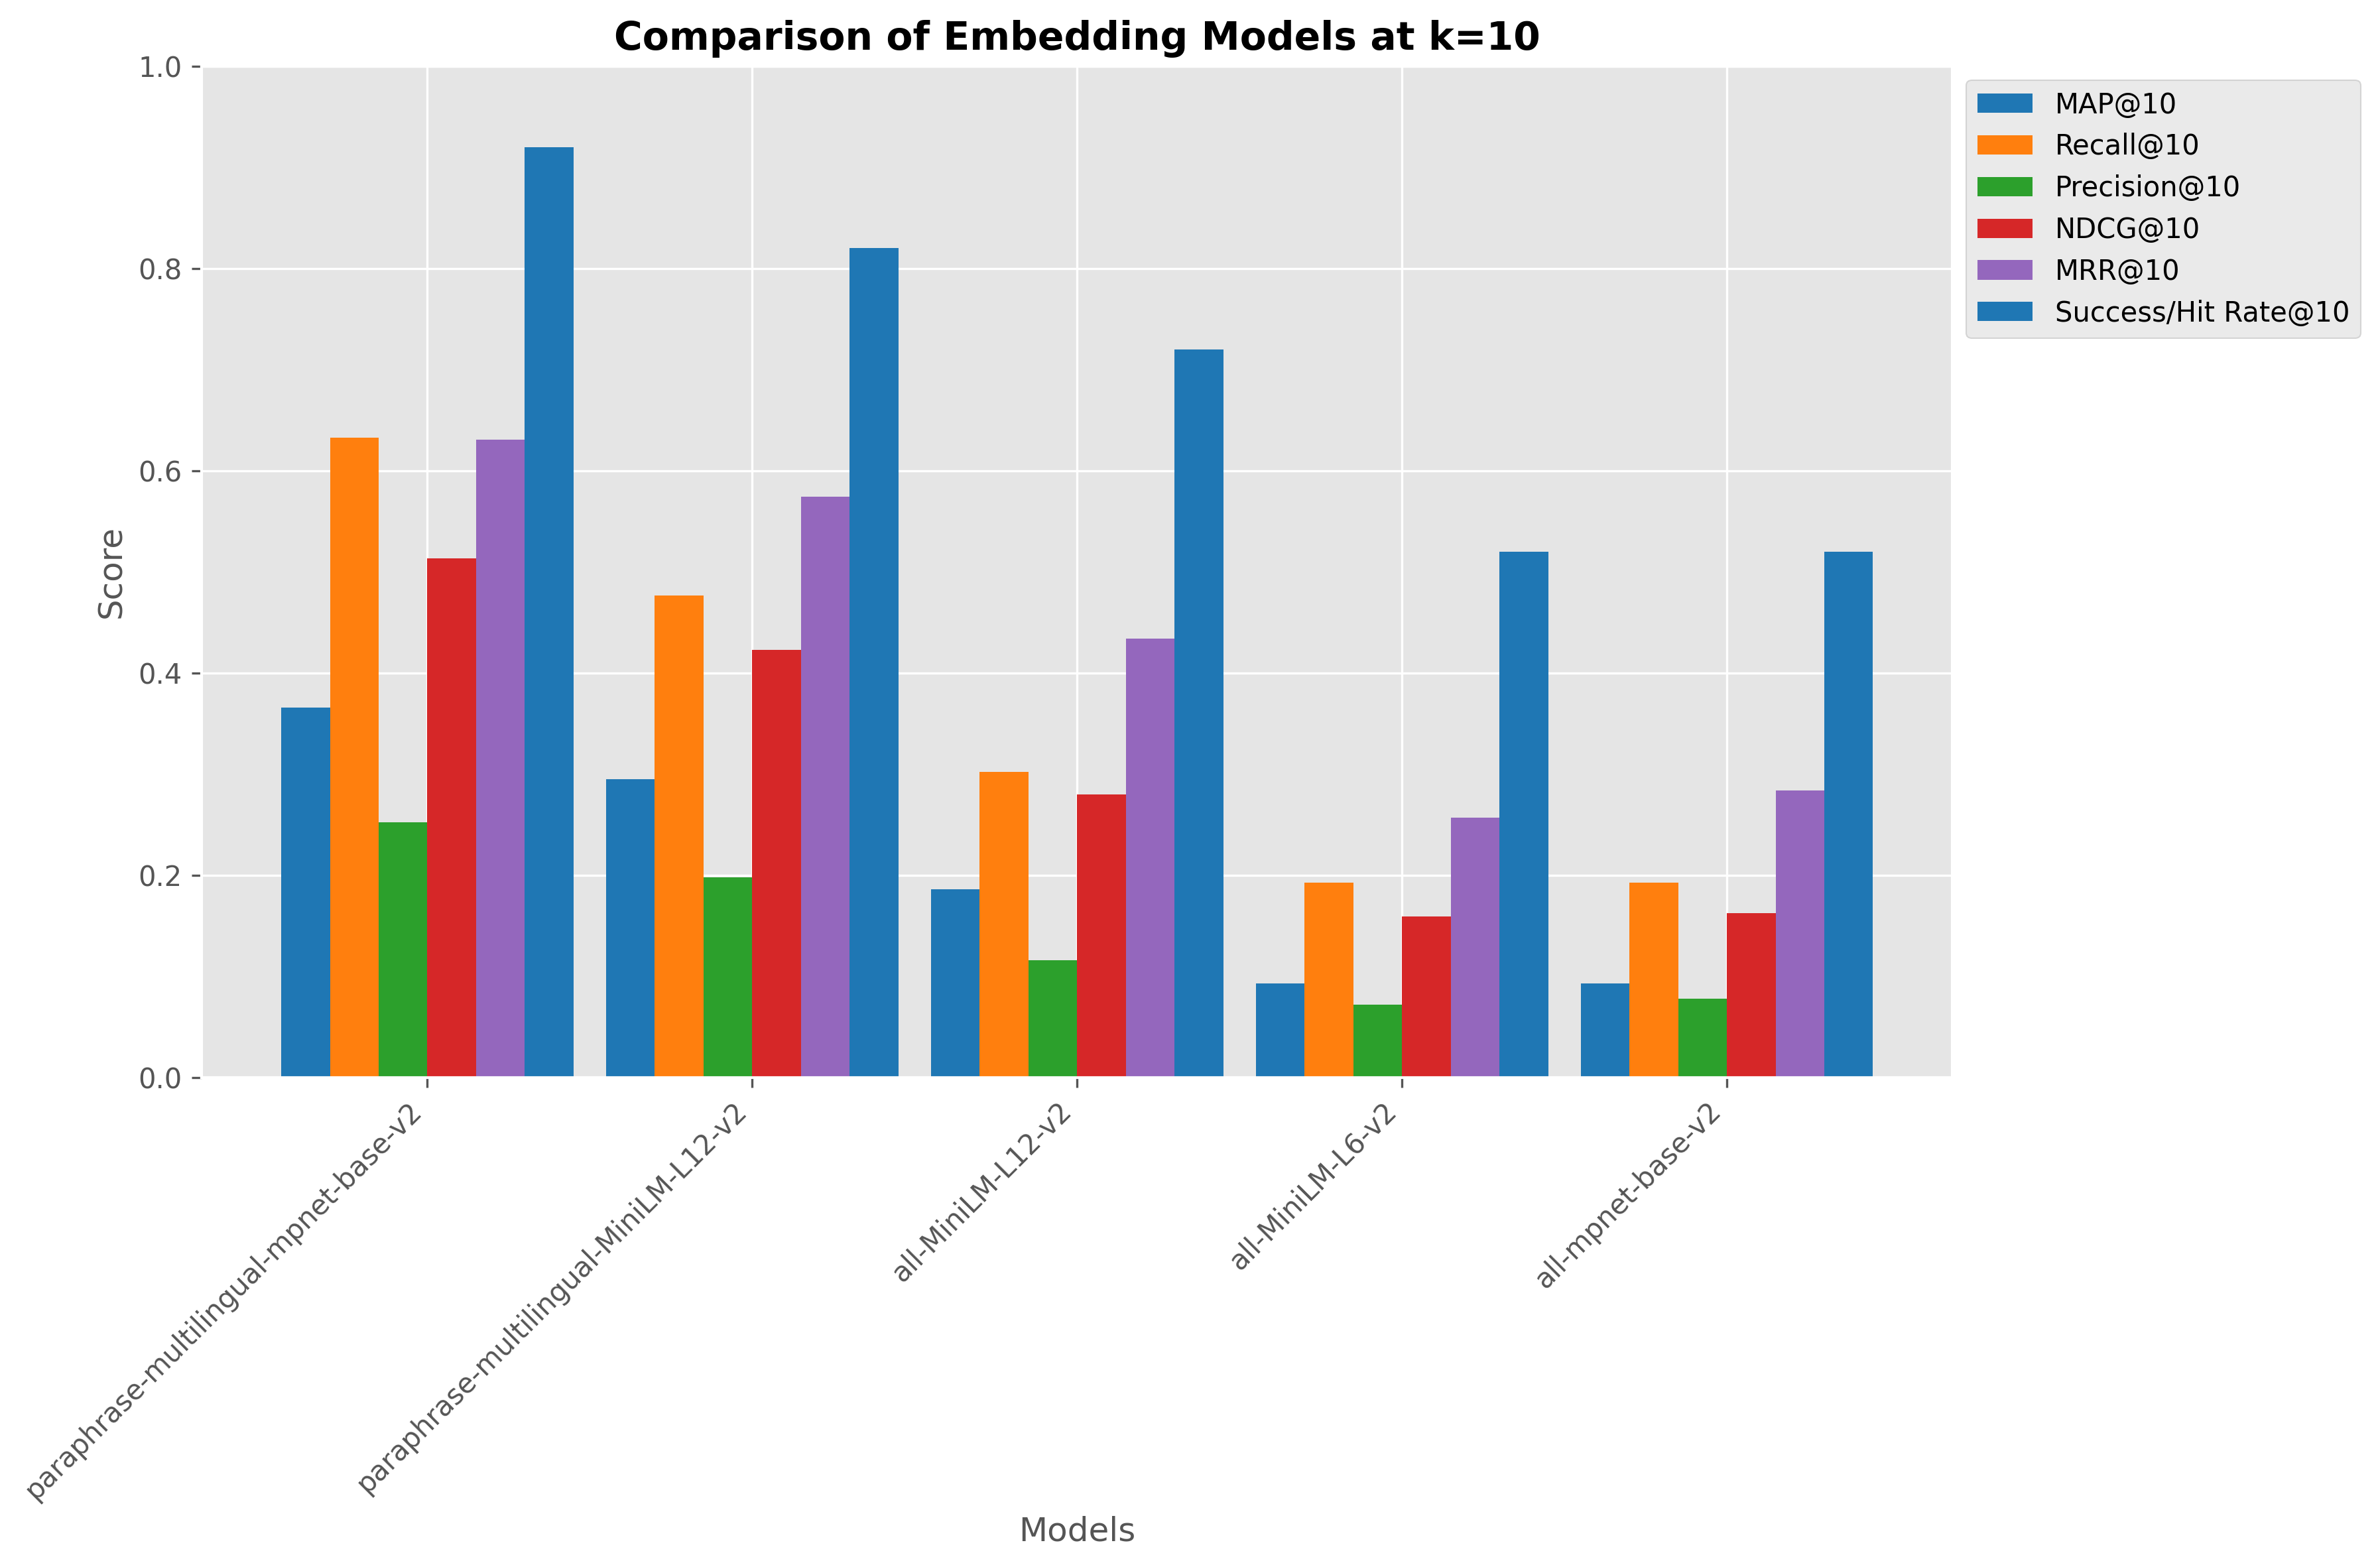
\includegraphics[width=0.92\linewidth]{results_law_tr_model_comparison.png}
\caption{Representative per-dataset metric profile generated automatically for the \texttt{law\_tr} benchmark.}\label{fig:results_law_tr_model_comparison}
\end{figure}

\subsection{Language Effect}\label{language-effect}

Under the shared evaluation setup in Section~\ref{shared-evaluation-setup}, the English and Turkish education corpora provide a controlled test of whether model behavior changes with corpus language. Table~\ref{tbl:language_effect_comparison} shows that the English results are tightly clustered, with all five models falling between 0.5020 and 0.6121 in \texttt{MAP@10}, whereas the Turkish results separate the roster much more sharply.

The monolingual English-oriented models (\texttt{M1}, \texttt{M2}, and \texttt{M4}) all decline substantially on \texttt{education\_tr}: \texttt{M1} drops by 0.4696, \texttt{M2} by 0.5183, and \texttt{M4} by 0.4206. By contrast, the multilingual models remain stable across languages: \texttt{M3} changes by only $-0.0144$, and \texttt{M5} is the only model that improves, rising by $+0.0104$. The evidence therefore suggests a language-level family tendency within this snapshot rather than a universal rule, and it also shows that \texttt{M4} remains competitive on \texttt{education\_eng}, so an English-oriented model can still be a strong choice when the corpus language matches the model family.

The practical implication is straightforward. For local retrieval deployment, language should be treated as a first-order selection variable: the best model for an English corpus is not necessarily the best model for a Turkish corpus, even when both corpora are evaluated under the same benchmark workflow. That is the main value of this result for the paper's fit-for-purpose claim.

\begin{table}[t]
\caption{Cross-language MAP@10 comparison within the education domain.}\label{tbl:language_effect_comparison}
\centering
\small
\begin{tabular}{@{}lccr@{}}
\toprule
Model & education\_eng MAP@10 & education\_tr MAP@10 & $\Delta$ (eng $\to$ tr) \\
\midrule
M1 & 0.6067 & 0.1371 & $-0.4696$ \\
M2 & 0.6074 & 0.0891 & $-0.5184$ \\
M3 & 0.5020 & 0.4876 & $-0.0144$ \\
M4 & 0.6121 & 0.1915 & $-0.4206$ \\
M5 & 0.5404 & 0.5508 & $+0.0104$ \\
\bottomrule
\end{tabular}
\end{table}

\subsection{Domain Effect Within Turkish}\label{domain-effect-within-turkish}

Under the shared evaluation setup in Section~\ref{shared-evaluation-setup}, Table~\ref{tbl:turkish_domain_comparison} isolates what changes when the corpus stays Turkish but the domain shifts from education to law/regulation.

\begin{table}[t]
\caption{Cross-domain comparison within the Turkish corpora.}\label{tbl:turkish_domain_comparison}
\centering
\small
\begin{tabular}{@{}l l r r r@{}}
\toprule
Model & Family & education\_tr MAP@10 & law\_tr MAP@10 & $\Delta$ (law $\!-\!$ education) \\
\midrule
M1 & English-oriented & 0.1371 & 0.0929 & $-0.0442$ \\
M2 & English-oriented & 0.0891 & 0.0928 & $+0.0037$ \\
M3 & Multilingual & 0.4876 & 0.2948 & $-0.1929$ \\
M4 & English-oriented & 0.1915 & 0.1863 & $-0.0052$ \\
M5 & Multilingual & 0.5508 & 0.3659 & $-0.1848$ \\
\bottomrule
\end{tabular}
\end{table}

The comparison shows a domain effect that is real but not uniform across models. The multilingual pair remains the strongest on both Turkish corpora, with \texttt{M5} and \texttt{M3} holding the top two positions in each dataset. However, both multilingual models lose substantially more absolute quality on \texttt{law\_tr} than the English-oriented models do: \texttt{M5} drops by 0.1849 and \texttt{M3} by 0.1928, while \texttt{M1} and \texttt{M4} decline only modestly and \texttt{M2} is essentially flat. The law/regulation corpus is therefore harder overall, but the domain shift interacts with model family rather than affecting all models equally. The practical implication is that Turkish-language benchmarking should not stop at a single Turkish corpus: a practitioner selecting an embedding model for legal or regulatory material should benchmark on that domain specifically, because Turkish-as-a-whole evidence can overstate performance on law/regulation documents.

\subsection{Quality-Speed Tradeoff}\label{quality-speed-tradeoff}

Table~\ref{tbl:quality_speed_summary} combines aggregate quality and timing evidence, and Figure~\ref{fig:results_quality_speed_tradeoff} makes the same tradeoff visible as a two-dimensional ranking. The points separate into three useful regimes. \texttt{M5} occupies the quality-leading end of the plot with the highest mean \texttt{MAP@10} at 0.4857, but it does so at a weighted latency of 60.55 ms/query and a throughput range of 14.1--15.1 chunks/s. \texttt{M1} anchors the speed-leading end with the lowest weighted latency at 28.54 ms/query and the highest throughput range of 48.0--57.1 chunks/s, but its mean \texttt{MAP@10} is only 0.2789. \texttt{M2} is the weakest aggregate choice in this snapshot because it combines the lowest mean \texttt{MAP@10} (0.2631) with the highest weighted latency (69.29 ms/query) and the slowest throughput range (3.9--8.6 chunks/s).

Within this roster, the multilingual models \texttt{M3} and \texttt{M5} provide the strongest cross-dataset retrieval quality, but speed is not a pure family effect because the monolingual \texttt{M2} is the slowest model overall. The more defensible snapshot-bounded reading is that multilingual models lead on average retrieval quality, while low latency is concentrated in \texttt{M1} and, to a lesser extent, \texttt{M4}. This pattern should not be treated as universal, however, because \texttt{M4} remains competitive on \texttt{education\_eng} and therefore shows that an English-oriented model can still be an effective choice when the corpus and deployment priority align.

The middle of the plot contains \texttt{M3} and \texttt{M4}, which are the most plausible compromise candidates when neither extreme is acceptable. \texttt{M3} is the stronger of the two on absolute retrieval quality, with mean \texttt{MAP@10} of 0.4281, while keeping latency close to \texttt{M4} at 35.05 ms/query versus 38.43 ms/query. \texttt{M4}, in turn, has the better average rank at 2.33, which suggests that it was more often near the top across the three datasets even though its mean \texttt{MAP@10} is lower than \texttt{M3}'s. The practical reading is therefore straightforward: \texttt{M5} is the best choice when retrieval effectiveness matters most, \texttt{M1} is the best choice when latency dominates, and \texttt{M3} or \texttt{M4} are the more balanced options for deployments that need an intermediate quality-speed compromise. On this evidence, no single model dominates all others jointly; the preferred embedding model depends on whether the practitioner values retrieval effectiveness, indexing cost, or interactive response time more strongly.

\begin{table}[t]
\caption{Aggregate quality-speed summary for the benchmarked embedding models.}\label{tbl:quality_speed_summary}
\centering
\small
\begin{tabular}{@{}lrrrr@{}}
\toprule
Model & Mean MAP@10 & Avg Rank & Weighted latency (ms/query) & Throughput range (chunks/s) \\
\midrule
M1 & 0.2789 & 3.67 & 28.54 & 48.0--57.1 \\
M2 & 0.2631 & 4.00 & 69.29 & 3.9--8.6 \\
M3 & 0.4281 & 3.00 & 35.05 & 44.8--48.2 \\
M4 & 0.3299 & 2.33 & 38.43 & 43.8--47.3 \\
M5 & 0.4857 & 2.00 & 60.55 & 14.1--15.1 \\
\bottomrule
\end{tabular}
\end{table}

\begin{figure}
\centering
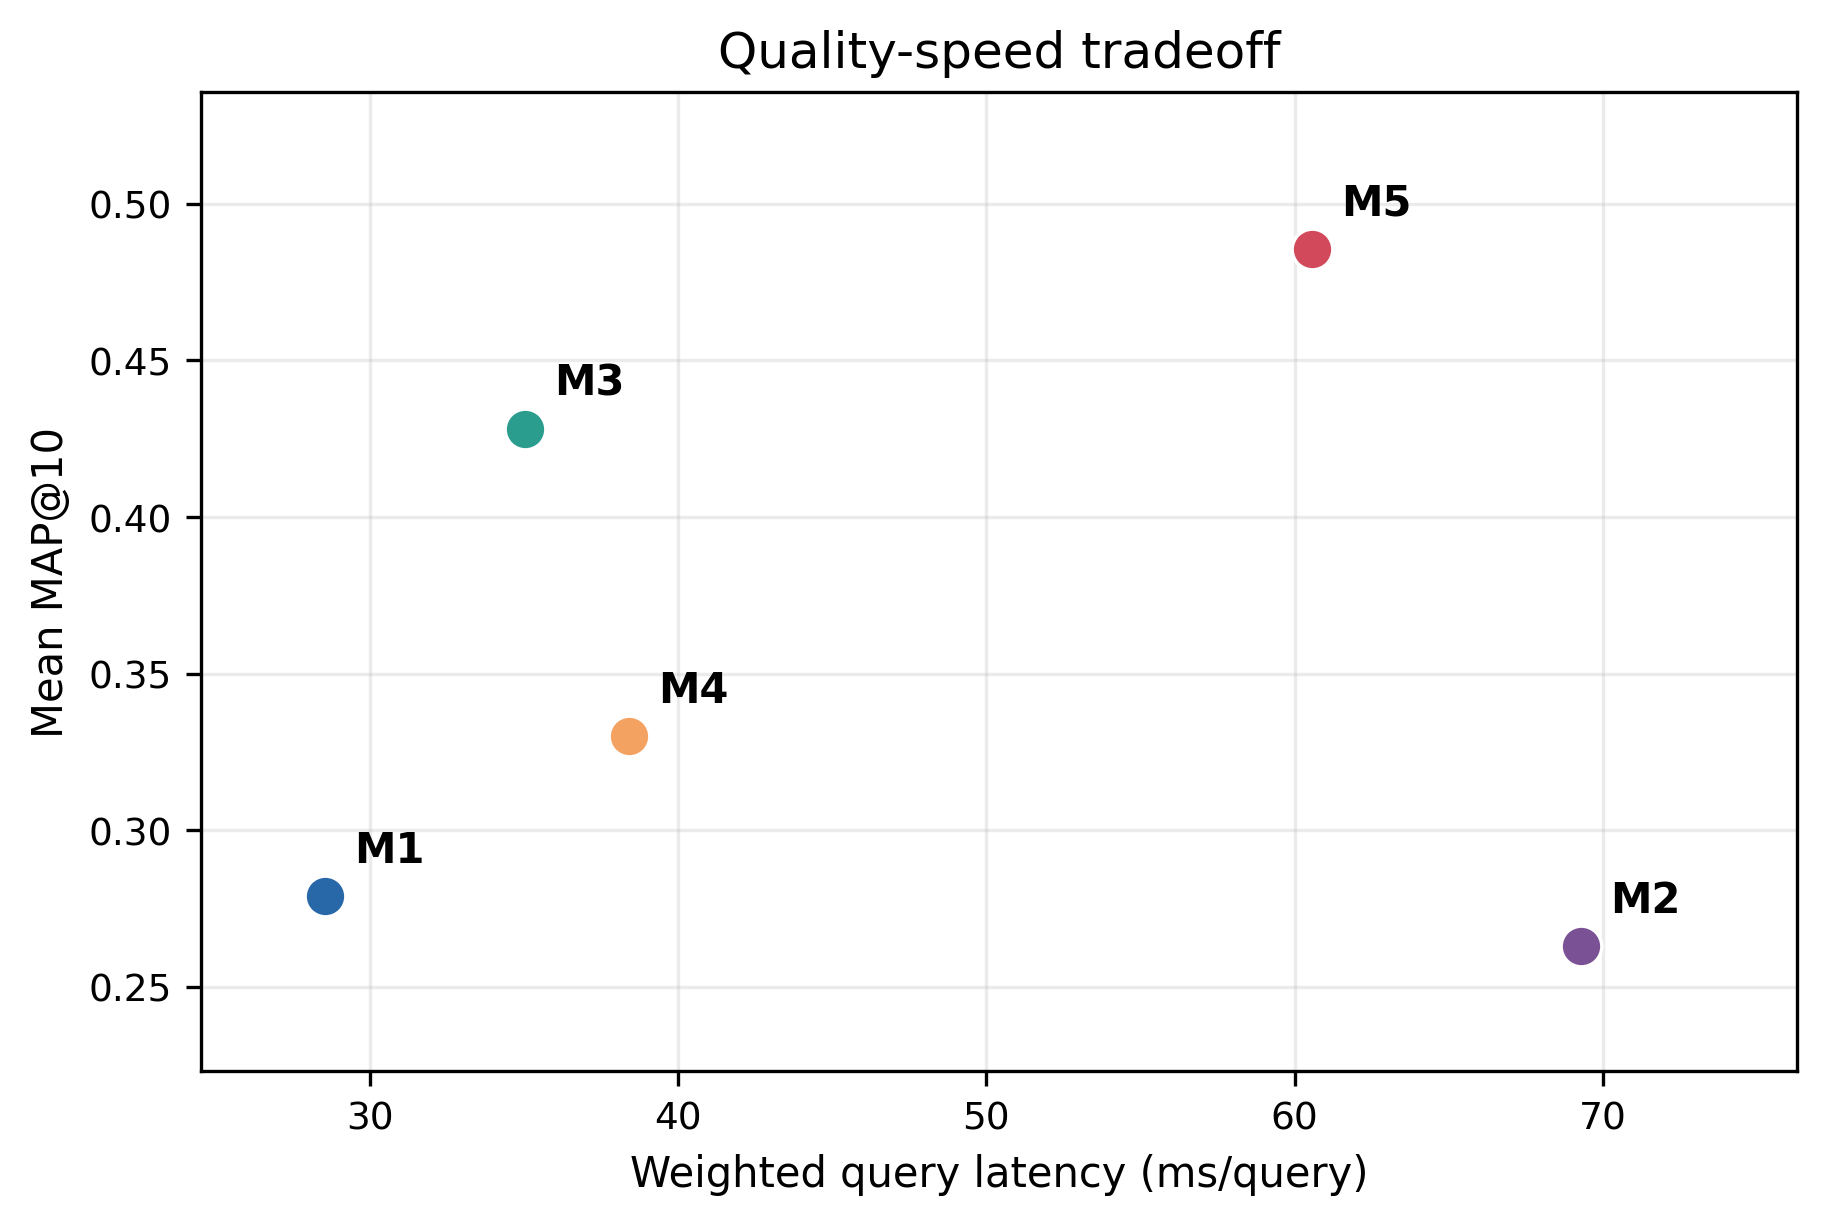
\includegraphics[width=0.92\linewidth]{results_quality_speed_tradeoff.png}
\caption{Quality-speed tradeoff scatter plot for the benchmarked embedding models.}\label{fig:results_quality_speed_tradeoff}
\end{figure}

\subsection{Statistical Decision Support}\label{statistical-decision-support}

The benchmark pipeline is intended not only to rank embedding models, but also to help a practitioner judge whether observed performance differences are strong enough to guide deployment decisions. For this reason, the automatically generated aggregate report includes statistical comparison outputs in addition to the descriptive metric tables and visual summaries reported above. In the current implementation, the aggregate report computes paired \texttt{MAP@10} comparisons between model pairs across datasets and a Friedman test over the five-model roster \citep{GitHub_RagRetrievalBench}. Table~\ref{tbl:statistical_decision_support} summarizes the decision-relevant outputs for the present three-dataset snapshot.

\begin{table}[t]
\caption{Statistical decision-support outputs generated by the aggregate report for the current snapshot.}\label{tbl:statistical_decision_support}
\centering
\small
\begin{tabular}{@{}llll@{}}
\toprule
Test & Comparison & Result & Decision-support reading \\
\midrule
Friedman & All five models & $\chi^2=3.47$, \texttt{p=0.483} & No global significant difference \\
Paired t-test & M5 vs. M4 & \texttt{p=0.339}, $d=0.83$ & Top-ranked pair not statistically separated \\
Paired t-test & M5 vs. M3 & \texttt{p=0.028}, $d=0.52$ & Significant under the report configuration \\
\bottomrule
\end{tabular}
\end{table}

These results should not be read as evidence that all models are interchangeable. Rather, they show how the pipeline separates descriptive performance differences from statistical decision support. The descriptive evidence remains practically useful: \texttt{M5} has the best mean \texttt{MAP@10}, the best average rank, and the strongest Turkish-corpus performance, while \texttt{M1} has the lowest weighted latency. The statistical output adds a cautionary layer: because the aggregate comparison is based on only three dataset-level paired observations, broad claims about universal model superiority are not warranted from this snapshot alone.

This distinction is central to the paper's contribution. A practitioner using the pipeline on a local corpus receives both model-selection evidence and uncertainty-oriented context. If a report shows large and statistically supported differences, the practitioner can treat the ranking as stronger deployment evidence. If, as in this snapshot, the global test is non-significant and the top-ranked pair is not statistically separated, the practitioner should prioritize fit-for-purpose criteria such as corpus language, domain, latency budget, indexing throughput, and tolerance for retrieval errors. In this way, the statistical report output supports the pipeline's goal: it helps users select a suitable embedding model for their own dataset and application requirements without overstating what the benchmark evidence can prove.

\section{Conclusion}\label{conclusion}

This paper presented a reusable, configuration-driven local benchmarking pipeline for corpus-specific embedding-model selection in RAG retrieval. The workflow takes an unlabeled local document collection as its starting point, constructs the queries and relevance judgments needed for evaluation, and produces the rankings, uncertainty estimates, and reports required for corpus-specific candidate comparison. Each collection is processed separately through ingestion, chunking, synthetic query generation, pooled qrels construction, multi-model retrieval evaluation, timing capture, and automated reporting. Its central research position is deliberately bounded: practitioners should not assume that one embedding model will be optimal for every corpus under their control. The three-corpus snapshot demonstrates how the workflow tests that assumption; it does not prove that a universal best model cannot exist.

For RQ1, the fixed snapshot shows that the configurable pipeline can produce inspectable, corpus-specific decision-support evidence. Separate reports for \texttt{education\_eng}, \texttt{education\_tr}, and \texttt{law\_tr} contain comparable retrieval metrics, timing summaries, query-level uncertainty, and preserved artifacts under the same five-model protocol. These reports support corpus-specific screening rather than a single cross-corpus selection rule.

For RQ2, the two education cases show language-associated ranking differences: English-oriented candidates lead \texttt{education\_eng}, whereas multilingual candidates lead \texttt{education\_tr}. This comparison does not establish a causal language effect because each language condition is represented by one corpus. For RQ3, the two Turkish cases instead show domain-associated stability: \texttt{M5} remains the quality-first candidate and \texttt{M3} the lower-latency alternative for both \texttt{education\_tr} and \texttt{law\_tr}. This stability does not show that domain is irrelevant; together, RQ2 and RQ3 illustrate why both shortlist change and shortlist stability should be examined through separate corpus runs.

For RQ4, the reports show that retrieval quality and operational priorities can produce different corpus-specific selections. They combine retrieval metrics with compound corpus embedding/index-insertion throughput, compound query-embedding/vector-search latency, and uncertainty intervals. What the uncertainty layer adds is visible in the demonstrated scenario: on \texttt{education\_eng} the quality advantage of the leading candidate over its runner-up lies within the paired bootstrap interval, so latency becomes the practical differentiator, whereas on both Turkish corpora the corresponding advantage is separated and the observed quality evidence guides the selection. The aggregate performance of \texttt{M5} remains secondary comparative context and does not override these corpus-level readings.

The current limitations also define clear directions for further evaluation. Human audit and judge calibration would strengthen the validation of synthetic queries and LLM-generated relevance judgments; controlled sensitivity studies would test dependence on retrieval and benchmark configuration; broader corpus and model coverage would assess transfer beyond the present snapshot; and repeated operational measurements would support stronger deployment-oriented performance claims.

The practical takeaway is that practitioners should not assume that a model selected from public benchmarks or a previous corpus will transfer unchanged to a new collection; materially different corpora should be evaluated using corpus-specific evidence, with aggregate results treated as secondary context and the final selection guided by project priorities.

\bibliographystyle{cas-model2-names}
\bibliography{refs}
\end{document}
